\documentclass[12pt]{article}
\UseRawInputEncoding
\usepackage[utf8]{inputenc}
\usepackage[T1]{fontenc}
\usepackage[catalan]{babel}
\usepackage{amsmath, amssymb, amsfonts}
\usepackage{geometry}
\usepackage{fancyhdr}
\usepackage{tikz}
\usetikzlibrary{matrix, calc}
\usepackage{tcolorbox}
\usepackage{lipsum}  
\usepackage[colorlinks=true, linkcolor=blue]{hyperref}
\usepackage{pgfkeys}
\usepackage{enumitem}
\usepackage[none]{hyphenat}
\usepackage{fancybox}
\setlength{\headheight}{15pt}

\sloppy

\geometry{a4paper, left=2cm, right=2cm, top=2.5cm, bottom=2.5cm}

\pagestyle{fancy}
\fancyhf{}
\fancyhead[L]{Matemàtiques}
\fancyhead[R]{Probabilitat}
\fancyfoot[L]{\href{mailto:orodri11@xtec.cat}{orodri11@xtec.cat}}
\fancyfoot[R]{\thepage}

\newtcolorbox{concept}[2][]{colback=blue!5!white, colframe=blue!75!black, fonttitle=\bfseries, title=Concepte, #1}
\newtcolorbox{exemple}[2][]{colback=green!5!white, colframe=green!75!black, fonttitle=\bfseries, title=Exemple, #1}
\newtcolorbox{exercici}[2][]{colback=yellow!5!white, colframe=yellow!75!black, fonttitle=\bfseries, title=Exercici, #1}

\newenvironment{solucio}{\begin{quote}\textbf{Solució:}}{\end{quote}}


\begin{document}

% Portada
\begin{titlepage}
    \centering
    {\Huge \textbf{Probabilitat \\ } \par}
    \vspace{1cm}
    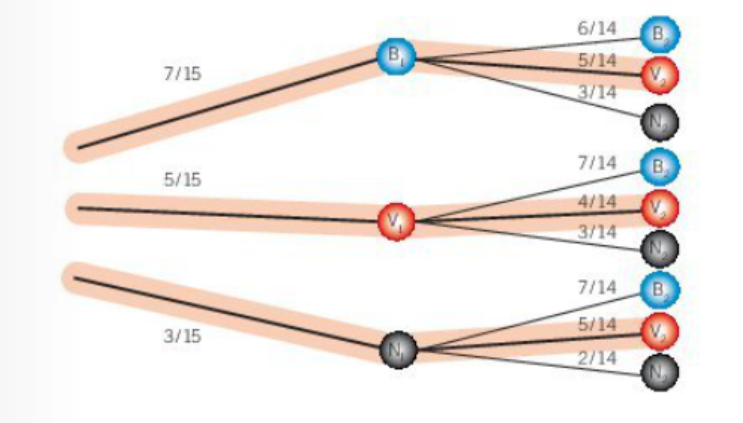
\includegraphics[width=0.5\textwidth]{prob.png}
    \vspace{1cm}
    \tableofcontents
\end{titlepage}

\newpage

\section{Introducció a la probabilitat}

\subsection*{Definició de probabilitat}

\begin{concept}[title=Probabilitat]
\noindent La probabilitat és una mesura que indica la possibilitat que un esdeveniment ocorri dins d'un conjunt d'esdeveniments possibles. Aquesta mesura es representa sempre amb un valor entre 0 i 1.
\end{concept}

\begin{concept}[title=Llei de Laplace] \noindent 
Fórmula clàssica (en contextos equiprobables):
\[
P(A) = \frac{\text{nombre de casos favorables a } A}{\text{nombre total de casos possibles}}
\]
\end{concept}

\subsection*{Espai mostral i esdeveniments}

\begin{concept}[title=Espai mostral] 
\noindent Espai mostral ($S$ o $\Omega$): Conjunt de tots els resultats possibles d'un experiment aleatori. Per exemple, en llançar un dau, l'espai mostral és $S = \{1, 2, 3, 4, 5, 6\}$.
\end{concept}

\begin{concept}[title=Esdeveniment] \noindent
Qualsevol subconjunt de l'espai mostral. Pot ser simple (un sol resultat) o compost (més d'un resultat). Per exemple, obtenir un nombre pare en llançar un dau és un esdeveniment compost $A = \{2, 4, 6\}$.
\end{concept}

\subsection*{Propietats de la probabilitat}

\begin{concept}[title=Esdeveniment cert] \noindent
La probabilitat d'un esdeveniment que sempre ocorre (com l'esdeveniment que inclou tot l'espai mostral) és 1.
\[
P(S) = 1
\]
\end{concept}

\begin{concept}[title=Esdeveniment impossible] \noindent
La probabilitat d'un esdeveniment que mai ocorre (com un esdeveniment buit) és 0.
\[
P(\emptyset) = 0
\]
\end{concept}

\begin{concept}[title=Unió d'esdeveniments]\noindent
Si tenim dos esdeveniments $A$ i $B$, la probabilitat que ocorri $A$ o $B$ (o ambdós) és:
\[
P(A \cup B) = P(A) + P(B) - P(A \cap B)
\]
Aquesta fórmula se simplifica a $P(A \cup B) = P(A) + P(B)$ si $A$ i $B$ són mútuament excloents (incompatibles, no poden ocórrer al mateix temps).
\end{concept}

\begin{concept} [title=Intersecció d'esdeveniments]\noindent
La probabilitat que ocorri $A$ i $B$ al mateix temps és:
\[
P(A \cap B) = P(A) \times P(B|A)
\]
on $P(B|A)$ és la probabilitat condicionada de $B$ donat $A$. Si $A$ i $B$ són independents, la fórmula es redueix a:
\[
P(A \cap B) = P(A) \times P(B)
\]
\end{concept}

\begin{concept} [title=Esdeveniment complementari (contrari)]\noindent
La probabilitat que no ocorri un esdeveniment $A$ és:
\[
P(\overline{A}) = 1 - P(A)
\]
on $\overline{A}$ és el complementari de $A$.
\end{concept}

\subsection*{Exemples}

\begin{exemple} \noindent 
Considerem el llançament d'una moneda. L'espai mostral és $S = \{\text{cara}, \text{creu}\}$. Si suposem que la moneda no està trucada, la probabilitat d'obtenir "cara" és:
\[
P(\text{cara}) = \frac{1}{2}
\]
\end{exemple}

\begin{exemple} \noindent Pensem en el llançament d'un dau de sis cares. Espai mostral: $S = \{1, 2, 3, 4, 5, 6\}$.

Esdeveniment $A$: Obtenir un nombre pare. 
\[
A = \{2, 4, 6\}
\]
\end{exemple}

\begin{exemple} \noindent 
\subsubsection*{Probabilitat d'un esdeveniment cert}
Exemple: En el llançament d'un dau, quina és la probabilitat d'obtenir un nombre entre 1 i 6?
\[
P(1 \leq x \leq 6) = 1
\]

\subsubsection*{Probabilitat d'un esdeveniment impossible}
Exemple: En el llançament d'un dau, quina és la probabilitat d'obtenir un 7?
\[
P(7) = 0
\]

\subsubsection*{Probabilitat de la unió d'esdeveniments}
Exemple: Suposem dos esdeveniments:
\begin{itemize}
    \item $A$: Obtenir un nombre menor que 3 en llançar un dau. $A = \{1, 2\}$
    \item $B$: Obtenir un nombre major que 4 en llançar un dau. $B = \{5, 6\}$
\end{itemize}

Quina és la probabilitat d'obtenir un nombre menor que 3 o un nombre major que 4? 
\[
P(A \cup B) = P(A) + P(B) = \frac{2}{6} + \frac{2}{6} = \frac{4}{6} = \frac{2}{3}
\]

\subsubsection*{Contrari o complementari}
Exemple: Si $A$ és obtenir un nombre pare en el llançament d'un dau, $A'$ seria obtenir un nombre imparell. Quina és la probabilitat d'obtenir un nombre imparell?
\[
P(A') = 1 - P(A) = 1 - \frac{3}{6} = \frac{1}{2}
\]
\end{exemple}


\section{Conceptes de probabilitat}

\begin{concept} [title=Experiment aleatori] \noindent Un experiment aleatori és qualsevol experiència que es pot repetir en les mateixes condicions però amb un resultat impredictible.

Per exemple, llançar un dau per veure quin nombre surt.
\end{concept}

\begin{concept} [title=Espai mostral]\noindent L'espai mostral és el conjunt de tots els possibles resultats d'un experiment aleatori.

Per exemple, si llancem un dau, l'espai mostral (anomenat $E$, $S$, $\Omega$ o $U$) és:
\[
\Omega = \{1, 2, 3, 4, 5, 6\}
\]
\end{concept}

\begin{concept} [title=Esdeveniment] \noindent Un esdeveniment és un subconjunt dels possibles resultats d'un espai mostral.

Per exemple, si llancem un dau, l'esdeveniment d'obtenir un nombre pare ($A = \{2, 4, 6\}$) és un esdeveniment compost. D'altra banda, que surti un 5 ($A = \{5\}$) és un esdeveniment elemental.
\end{concept}

\begin{concept} [title=Esdeveniment elemental]\noindent Un esdeveniment elemental és quan l'esdeveniment està format per un únic resultat, és a dir, un únic element de l'espai mostral.
\end{concept}

\begin{concept} [title=Esdeveniment compost]\noindent Un esdeveniment compost és quan l'esdeveniment està format per diversos resultats, és a dir, més d'un element de l'espai mostral.
\end{concept}

\subsection*{Exemples d'espai mostral}

\begin{exemple} [title=Llançament d'una moneda] \noindent Quan llancem una moneda, hi ha dues possibilitats: cara (C) o creu (X). \\

Espai mostral:
\[
E_1 = \{C, X\}
\]
\end{exemple}

\begin{exemple}[title=Llançament d'un dau] \noindent Si llancem un dau de sis cares, les possibles sortides són els nombres del 1 al 6. \\

Espai mostral:
\[
E_2 = \{1, 2, 3, 4, 5, 6\}
\]
\end{exemple}

\begin{exemple} [title=Llançament de dues monedes] \noindent Si llancem dues monedes, les combinacions possibles són: cara-cara (CC), cara-creu (CX), creu-cara (XC) i creu-creu (XX). \\

Espai mostral:
\[
E_3 = \{CC, CX, XC, XX\}
\]
\end{exemple}

\begin{exemple} [title=Elecció d'un gelat]\noindent Les combinacions possibles de dos sabors diferents de gelat són: vainilla-xocolata (VX), vainilla-maduixa (VM), i xocolata-maduixa (XM). \\

Espai mostral:
\[
E_4 = \{VX, VM, XM\}
\]
\end{exemple}

\begin{exemple} [title=Combinacions d'un cadenat]\noindent Per a un cadenat amb un codi de 3 xifres, on cada xifra pot ser del 0 al 9, tenim 10 opcions per a cada xifra. Això ens dona un total de $10 \times 10 \times 10 = 1000$ combinacions possibles. \\

Espai mostral:
\[
E_5 = \{000, 001, 002, \dots, 999\}
\]
\end{exemple}

\begin{exemple}[title=Elecció de roba] \noindent Si una persona té 3 camises i 2 pantalons, el nombre de combinacions possibles és $3 \times 2 = 6$. \\

Les combinacions possibles són:
\[
E_1 = \{\text{blava-negre}, \text{blava-gris}, \text{vermella-negre}, \text{vermella-gris}, \text{groga-negre}, \text{groga-gris}\}
\]
\end{exemple}

\begin{exemple} [title=Llançament de dos daus]\noindent Quan llancem dos daus de sis cares, les combinacions possibles són $6 \times 6 = 36$. \\

L'espai mostral serà:
\[
E_2 = \{(1, 1), (1, 2), (1, 3), \dots, (6, 6)\}
\]
\end{exemple}

\begin{exemple}[title=Elecció d'una pizza] \noindent Si escollim 2 ingredients entre 4 possibles (pernil, bolets, pebrots, olives), el nombre de combinacions possibles és $C(4, 2) = 6$. \\

L'espai mostral serà:
\[
E_3 = \left\{
\begin{aligned}
    &\text{pernil-bolets}, \text{pernil-pebrots}, \text{pernil-olives}, \\
    &\text{bolets-pebrots}, \text{bolets-olives}, \text{pebrots-olives}
\end{aligned}
\right\}
\]

\end{exemple}

\begin{exemple}[title=Selecció de llibres] \noindent Si un estudiant vol escollir 3 llibres entre 5 possibles, el nombre de combinacions possibles és $C(5, 3) = 10$. \\

L'espai mostral serà:
\[
E_4 = \left\{
\begin{aligned}
    &\{Llibre_1, Llibre_2, Llibre_3\}, \{Llibre_1, Llibre_2, Llibre_4\}, \\
    &\dots, \{Llibre_3, Llibre_4, Llibre_5\}
\end{aligned}
\right\}
\]

\end{exemple}

\begin{exemple}[title=Codi de colors] \noindent Si tenim 4 colors i formem seqüències de 3 colors amb repetició, el nombre de combinacions possibles és $4^3 = 64$. \\

L'espai mostral serà:
\[
E_5 = \{(\text{vermell}, \text{vermell}, \text{vermell}), (\text{vermell}, \text{vermell}, \text{blau}), \dots, (\text{groc}, \text{groc}, \text{groc})\}
\]
\end{exemple}

\subsection*{Exercicis proposats espai mostral}

\begin{exercici} \noindent 
\textbf{1. Gustos de batut.} Una cafeteria ofereix batuts amb les següents opcions de fruita: poma, plàtan, maduixa i taronja. Si un client pot escollir 2 fruites diferents per al seu batut, quines combinacions possibles hi ha? Escriu l'espai mostral.
\end{exercici}

\begin{exercici} \noindent 
\textbf{2. Selecció d'equips.} En un torneig esportiu, hi ha 5 equips: A, B, C, D i E. Si se seleccionen 2 equips per jugar la final, quines combinacions possibles hi ha? Escriu l'espai mostral.
\end{exercici}

\begin{exercici} \noindent 
\textbf{3. Combinacions de begudes.} En una festa, ofereixen 4 tipus de begudes: aigua, refresc, suc i cervesa. Si un convidat decideix agafar 2 begudes diferents, quines combinacions pot tenir? Escriu l'espai mostral.
\end{exercici}

\begin{exercici} \noindent 
\textbf{4. Llançament de monedes.} Imagina que llancem 3 monedes consecutivament. Quines són totes les seqüències possibles de cares i creus? Escriu l'espai mostral.
\end{exercici}

\begin{exercici} \noindent 
\textbf{5. Selecció de cursos.} Una universitat ofereix 5 cursos optatius diferents. Si un estudiant pot escollir 3 cursos per al semestre, quants conjunts diferents de cursos pot escollir? Escriu l'espai mostral.
\end{exercici}

\begin{exercici} \noindent 
\textbf{6. Combinacions de postres.} En un restaurant, hi ha 4 postres disponibles: pastís, gelat, fruita i flam. Si un comensal decideix menjar 2 postres diferents, quines combinacions pot tenir? Escriu l'espai mostral.
\end{exercici}

\begin{exercici} \noindent 
\textbf{7. Selecció de llibres.} Una llibreria ofereix 3 llibres diferents de ciència-ficció, 2 de misteri i 4 d'història. Si un client decideix comprar 1 llibre de cada categoria, quantes combinacions diferents pot tenir? Escriu l'espai mostral.
\end{exercici}

\begin{exercici} \noindent 
\textbf{8. Selecció de colors.} Tens una paleta de colors amb 5 colors diferents. Si vols pintar una habitació amb 2 colors diferents (un per a les parets i un altre per al sostre), quines combinacions pots tenir? Escriu l'espai mostral.
\end{exercici}

\begin{exercici} \noindent 
\textbf{9. Combinacions de música.} Tens 4 àlbums de rock i 3 àlbums de jazz. Si vols escoltar 1 àlbum de cada gènere, quines combinacions pots tenir? Escriu l'espai mostral.
\end{exercici}

\begin{exercici} \noindent 
\textbf{10. Selecció d'esports.} Una escola ofereix 4 esports diferents: futbol, bàsquet, tenis i voleibol. Si un estudiant pot practicar 2 esports diferents durant l'any, quines combinacions possibles hi ha? Escriu l'espai mostral.
\end{exercici}

\subsection*{Propietats de la probabilitat}

\begin{concept}[title=Propietats] \noindent
\par
\begin{itemize}
    \item La probabilitat de qualsevol esdeveniment està entre 0 i 1:
    \[
    0 \leq P(A) \leq 1
    \]
    \item La probabilitat d'ocurrència de tot l'espai mostral és 1:
    \[
    P(\Omega) = 1
    \]
    \item La probabilitat de l'esdeveniment oposat és:
    \[
    P(A^c) = 1 - P(A)
    \]
    \item Si $A$ i $B$ són esdeveniments incompatibles:
    \[
    P(A \cup B) = P(A) + P(B)
    \]
    \[
    P(A \cap B) = 0
    \]
    \item Si $A$ i $B$ són esdeveniments compatibles:
    \[
    P(A \cup B) = P(A) + P(B) - P(A \cap B)
    \]
    \item Si $A$ i $B$ són esdeveniments independents:
    \[
    P(A \cap B) = P(A) \cdot P(B)
    \]
    \item Si $A$ i $B$ són esdeveniments dependents:
    \[
    P(A \cap B) = P(A) \cdot P(B \mid A)
    \]
\end{itemize}
\end{concept}


\subsection*{Esdeveniments}

\begin{concept} [title=Unió d'esdeveniments] \noindent La unió dels esdeveniments $A$ i $B$ és quan ocorre l'esdeveniment $A$ o l'esdeveniment $B$. Es representa per: $A \cup B$.  \\

\textbf{Exemple:}  
Si $A$ és l'esdeveniment "sortir nombre primer en llançar un dau" i $B$ és l'esdeveniment "sortir nombre senar", tenim:  
\[
A = \{2, 3, 5\}, \quad B = \{1, 3, 5\}
\]  
Per tant:  
\[
A \cup B = \{1, 2, 3, 5\}
\]
\end{concept}

\begin{concept} [title=Intersecció d'esdeveniments] \noindent La intersecció dels esdeveniments $A$ i $B$ és quan ocorre l'esdeveniment $A$ i l'esdeveniment $B$ de forma simultània. Es representa per: $A \cap B$.  \\

\textbf{Exemple:}  
Amb l'exemple anterior:  
\[
A \cap B = \{3, 5\} \quad \text{(nombres primers i senars alhora)}
\]  
Quan $A \cap B = \emptyset$, els esdeveniments són incompatibles (per exemple, nombre senar i parell).  
Quan $A \cap B \neq \emptyset$, els esdeveniments són compatibles.
\end{concept}

\begin{concept} [title=Esdeveniments dependents] \noindent Dos esdeveniments compatibles són independents quan l'ocurrència d'un no influeix en la de l'altre.  \\

\textbf{Exemple:}  
La probabilitat que plogui demà és independent de la probabilitat que guanyi el Barça a l'Espanyol avui.  

Dos esdeveniments són dependents quan l'ocurrència d'un influeix en l'altra. \\ 

\textbf{Exemple:}  
La probabilitat de patir un accident de trànsit depèn d'haver begut alcohol o no.
\end{concept}

\begin{concept} [title=Esdeveniment contrari]\noindent L'esdeveniment contrari de $A$ és l'esdeveniment que té lloc quan no ocorre $A$. Es representa per $A^c$.  \\

\textbf{Exemple:}  
Si $A$ és l'esdeveniment "sortir nombre primer en llançar un dau", amb $A = \{2, 3, 5\}$, l'esdeveniment contrari és:  
\[
A^c = \{1, 4, 6\}
\]  
La probabilitat de l'esdeveniment contrari és:  
\[
P(A^c) = 1 - P(A)
\]

\textbf{Exemple:}  
Si la probabilitat de pluja per demà és del 20\%, la probabilitat que no plogui és $100\% - 20\% = 80\%$.
\end{concept}

\subsection*{Independència d'esdeveniments}

\begin{concept} [title=Esdeveniments independents] \noindent Dos esdeveniments $A$ i $B$ són independents si el fet que un ocorri no afecta la probabilitat que l'altre ocorri. \\

Matemàticament:  
\[
P(A \mid B) = P(A) \quad \text{o equivalentment,} \quad P(A \cap B) = P(A) \cdot P(B)
\]
\end{concept}

\begin{concept} [title=Propietats dels esdeveniments independents] \noindent  
\begin{itemize}
    \item Si $A$ i $B$ són independents, llavors $A^c$ (el complementari de $A$) i $B$ també són independents, i viceversa.
    \item La independència és simètrica: si $A$ és independent de $B$, llavors $B$ també és independent de $A$.
    \item Dos esdeveniments independents no són necessàriament incompatibles. De fet, dos esdeveniments mútuament excloents no poden ser independents (a menys que la probabilitat d'algun d'ells sigui zero).
\end{itemize}
\end{concept}

\begin{concept} [title=Diferència entre esdeveniments independents i incompatibles] \noindent
\begin{itemize}
    \item \textbf{Esdeveniments independents:}  
    Dos esdeveniments són independents si el fet que un ocorri no afecta la probabilitat que l'altre ocorri. La seva intersecció no és nul·la:  
    \[
    P(A \cap B) = P(A) \cdot P(B)
    \]
    \item \textbf{Esdeveniments incompatibles o mútuament excloents:}  
    Dos esdeveniments són mútuament excloents si no poden ocórrer al mateix temps. És a dir, la seva intersecció és nul·la:  
    \[
    P(A \cap B) = 0
    \]
\end{itemize}
\end{concept}

\begin{exemple} [title=Exemples]     
\noindent
\textbf{Esdeveniments independents:}  
\begin{itemize}
    \item Llançar una moneda i un dau. El resultat del llançament de la moneda no té cap efecte en el resultat del dau, i viceversa.
    \item Triar una targeta d'una baralla i després retornar-la, i triar una altra targeta. Les dues eleccions són independents perquè la primera elecció no afecta la segona.
\end{itemize}

\textbf{Esdeveniments incompatibles:}  
\begin{itemize}
    \item En llançar un dau, obtenir un nombre parell i obtenir un 3 són esdeveniments mútuament excloents, ja que no poden passar al mateix temps.
    \item En una cursa, un corredor guanyant i un altre corredor quedant en primer lloc també són mútuament excloents. Només pot haver-hi un primer lloc.
\end{itemize}
\end{exemple}

\subsection*{Freqüències i probabilitats d'un esdeveniment}

\begin{concept} [title=Freqüència absoluta i relativa] \noindent Quan fem un experiment aleatori, podem mesurar dos tipus de freqüències:  
\begin{itemize}
    \item \textbf{Freqüència absoluta:} És el número de vegades que té lloc un esdeveniment $A$, denotat per $f(A)$.
    \item \textbf{Freqüència relativa:} És el quocient entre el número de vegades que es produeix l'esdeveniment i el número total d'experiments realitzats, denotat per $h(A)$:
    \[
    h(A) = \frac{f(A)}{\text{nombre total d'experiments}}
    \]
\end{itemize}
\textbf{Exemple:}  
Si llancem una moneda 20 vegades i surt cara (C) 12 vegades:  
\[
f(C) = 12, \quad h(C) = \frac{12}{20} = 0,6
\]
En percentatge:  
\[
0,6 \times 100 = 60\%
\]
\end{concept}

\begin{exercici} \noindent 
\textbf{Experiment pràctic:}  
Llança una moneda 20 vegades i registra el nombre de cares i de creus. Calcula la freqüència absoluta i relativa de cada esdeveniment.
\end{exercici}

\begin{concept} [title=Assignació de probabilitats als esdeveniments] \noindent Les probabilitats dels esdeveniments en experiments aleatoris es poden assignar de dues maneres principals:  
\begin{itemize}
    \item \textbf{A priori:} Es fa servir un model matemàtic per assignar una probabilitat a cada esdeveniment. Un exemple és la regla de Laplace:  
    \[
    P(A) = \frac{\text{nombre de casos favorables}}{\text{nombre de casos possibles}}
    \]
    \item \textbf{A posteriori:} S'assignen les probabilitats utilitzant la freqüència relativa obtinguda d'experiments reals. Quan es repeteix un gran nombre de vegades l'experiment, la freqüència relativa tendeix a la probabilitat real.
\end{itemize}
\end{concept}

\newpage

\section{Probabilitat Condicional}

\begin{concept}  [title=Definició] \noindent La probabilitat condicional ens permet calcular la probabilitat d'un esdeveniment $A$, tenint en compte que un altre esdeveniment $B$ ja ha ocorregut. Es denota com $P(A \mid B)$ i es defineix com la probabilitat que ocorri $A$ assumint que $B$ ja ha ocorregut. La fórmula per calcular la probabilitat condicional és:
\[
P(A \mid B) = \frac{P(A \cap B)}{P(B)}
\]
on:  
\begin{itemize}
    \item $P(A \mid B)$ és la probabilitat condicional d'$A$ donat $B$.
    \item $P(A \cap B)$ és la probabilitat que ocorrin simultàniament $A$ i $B$, també coneguda com la probabilitat de la intersecció de $A$ i $B$.
    \item $P(B)$ és la probabilitat que ocorri l'esdeveniment $B$.
\end{itemize}
\end{concept}

\begin{exemple}  [title=Exemple 1]  \noindent 
\textbf{Botiga d'electrònica:}  
Imagina que estàs en una botiga d'electrònica. A la botiga hi ha dos tipus de productes que t'interessen: mòbils (A) i auriculars (B). Les dades són les següents:

\begin{itemize}
    \item La probabilitat que un client compri un mòbil és $P(A) = 0.6$.
    \item La probabilitat que un client compri auriculars és $P(B) = 0.5$.
    \item La probabilitat que un client compri tant un mòbil com auriculars és $P(A \cap B) = 0.3$.
\end{itemize}
Pregunta: Si saps que un client ha comprat auriculars, quina és la probabilitat que també hagi comprat un mòbil? \\

\textbf{Solució:}  
Utilitzant la fórmula de probabilitat condicional:
\[
P(A \mid B) = \frac{P(A \cap B)}{P(B)} = \frac{0.3}{0.5} = 0.6
\]
Així que la probabilitat que un client que ha comprat auriculars també hagi comprat un mòbil és $0.6$ o $60\%$.
\end{exemple}

\begin{exemple}  [title=Exemple 2] \noindent 
\textbf{Estudiants jugant a futbol i bàsquet:}  
Suposem que en una classe de 30 estudiants, 10 estudiants juguen a futbol i 15 estudiants juguen a bàsquet. 5 d'aquests estudiants juguen tant a futbol com a bàsquet. Si un estudiant és seleccionat a l'atzar i es descobreix que juga a bàsquet, quina és la probabilitat que també jugui a futbol? \\

\textbf{Solució:}  
Utilitzant la fórmula de probabilitat condicional:
\[
P(F \mid B) = \frac{P(F \cap B)}{P(B)} = \frac{5/30}{15/30} = \frac{1}{3}
\]
Així que, si sabem que un estudiant juga a bàsquet, la probabilitat que també jugui a futbol és $\frac{1}{3}$ o aproximadament 33.33\%.
\end{exemple}

\newpage

\section{Teorema de la Probabilitat Total}

\begin{concept}  [title=Introducció] \noindent
En el món real, ens trobem sovint amb situacions on un esdeveniment pot succeir a través de diversos camins o causes. Imagina, per exemple, que vols calcular la probabilitat que un estudiant aprovi un examen. Aquesta probabilitat pot dependre de si l'estudiant ha estudiat o no, i de si ha assistit a classes particulars. \\

El teorema de la probabilitat total ens ajuda a calcular la probabilitat d'un esdeveniment tenint en compte totes les possibles causes.
\end{concept}

\begin{concept}  [title=Definició] \noindent
    El teorema de la probabilitat total s'expressa mitjançant la fórmula següent:
    \[
    P(A) = \sum_{i=1}^{n} P(A \mid B_i) \cdot P(B_i)
    \]
    On:
    \begin{itemize}
        \item \( P(A \mid B_i) \) és la probabilitat condicional de \( A \) donat que \( B_i \) ha ocorregut.
        \item \( P(B_i) \) és la probabilitat de que l'esdeveniment \( B_i \) ocorri.
    \end{itemize}
    La versió estesa d'aquesta fórmula és:
    \[
    P(A) = P(A \mid B_1) \cdot P(B_1) + P(A \mid B_2) \cdot P(B_2) + \cdots + P(A \mid B_n) \cdot P(B_n)
    \]
\end{concept}

\begin{exemple}  [title=Exemple 1]  \noindent Suposa que tens una bossa amb 100 daus. D'aquests:

\begin{itemize}
    \item 80 són daus normals i equilibrats.
    \item 20 estan trucats perquè els nombres parells surtin amb una probabilitat més alta.
\end{itemize}

Quan prens un dau a l'atzar de la bossa i el llances, hi ha dues possibles situacions:

\begin{itemize}
    \item Si agafes un dau normal, la probabilitat d'obtenir un nombre parell és del 50\%.
    \item Si agafes un dau trucat, la probabilitat d'obtenir un nombre parell és del 70\%.
\end{itemize}

El teorema de la probabilitat total ens permet calcular la probabilitat composta d'obtenir un nombre parell quan es tira un dau tret a l'atzar de la bossa. \\

Això es fa ponderant la probabilitat d'obtenir un nombre parell de cada dau pel nombre de daus d'aquell tipus, i després sumant les dues quantitats.

\end{exemple}

\begin{exemple} \noindent Aquest càlcul es representa amb la fórmula:

\[
P(A) = P(A \mid \text{dau normal}) \cdot P(\text{dau normal}) + P(A \mid \text{dau trucat}) \cdot P(\text{dau trucat})
\]

Tenim:

\[
P(A \mid \text{dau normal}) = 0.5, \quad P(\text{dau normal}) = \frac{80}{100} = 0.8
\]
\[
P(A \mid \text{dau trucat}) = 0.7, \quad P(\text{dau trucat}) = \frac{20}{100} = 0.2
\]

Substituint aquestes dades a la fórmula:

\[
P(A) = 0.5 \times 0.8 + 0.7 \times 0.2 = 0.4 + 0.14 = 0.54
\]\\

D'aquesta manera, la probabilitat composta d'obtenir un nombre parell, després de llançar un dau tret a l'atzar de la bossa, és del 54\%.
\end{exemple}

\begin{exemple} [title=Exemple 2] \noindent 
Imagina que en una escola, el 60\% dels estudiants fan classes particulars (anomenem aquest grup \(B_1\)) i el 40\% no en fan (grup \(B_2\)). Dels estudiants que fan classes particulars, un 90\% aproven l'examen (probabilitat d'aprovar donat que són de \(B_1\)). Dels que no en fan, un 70\% aproven (probabilitat d'aprovar donat que són de \(B_2\)).\\

Quina és la probabilitat que un estudiant triat a l'atzar aprovi l'examen?

Fent servir el teorema de la probabilitat total:

\[
P(\text{Aprovar}) = P(\text{Aprovar} \mid B_1) \cdot P(B_1) + P(\text{Aprovar} \mid B_2) \cdot P(B_2)
\]

Ara, substituïm les dades donades:

\[
P(\text{Aprovar}) = 0.9 \times 0.6 + 0.7 \times 0.4
\]

Després de calcular, obtindrem que la probabilitat que un estudiant triat a l'atzar aprovi l'examen és del 82\%.
\end{exemple}

\begin{concept} [title=Conclusió] \noindent
El teorema de la probabilitat total és una eina que s'utilitza quan volem determinar la probabilitat d'un esdeveniment que pot succeir a través de múltiples vies o causes. En ciències socials, aquest teorema pot ser utilitzat en àrees com l'economia, la sociologia, la psicologia, entre altres, per entendre millor la probabilitat d'esdeveniments complexos que depenen de diversos factors.

Recorda sempre considerar totes les vies possibles quan utilitzis aquest teorema, i assegura't que les probabilitats condicionals i les probabilitats dels esdeveniments de la partició són correctes i completen l'espai de mostra.
\end{concept}

\section{Teorema de Bayes}

\begin{concept} [title=Definició] \noindent
El teorema de Bayes és una fórmula matemàtica que permet calcular la probabilitat d'un esdeveniment basat en el coneixement previ que està relacionat amb l'esdeveniment. És un concepte fonamental en la teoria de la probabilitat i proporciona una manera de revisar les nostres creences a la llum de noves dades o informació.

La fórmula del teorema de Bayes és:

\[
P(A \mid B) = \frac{P(B \mid A) \cdot P(A)}{P(B)}
\]

Això és el mateix que:

\[
P(A \mid B) = \frac{P(B \cap A)}{P(B)}
\]

on:
\begin{itemize}
    \item \( P(A \mid B) \) és la probabilitat posterior d'A donat que B és cert. Això és el que volem calcular.
    \item \( P(B \mid A) \) és la probabilitat de B donat que A és cert. Aquesta és la informació que generalment coneixem.
    \item \( P(A) \) és la probabilitat a priori d'A. Aquesta és la nostra creença original sobre A abans de tenir més informació.
    \item \( P(B) \) és la probabilitat total de B.
\end{itemize}

Si no tenim \( P(B) \), podem calcular-la mitjançant la regla de la probabilitat total. Si tenim diversos esdeveniments \( A_1, A_2, \dots, A_n \) que són mútuament exclusius i col·lectivament exhaustius (és a dir, un i només un d'ells pot ocórrer i la seva unió cobreix tot l'espai mostral), llavors:

\[
P(B) = P(B \mid A_1) \cdot P(A_1) + P(B \mid A_2) \cdot P(A_2) + \dots + P(B \mid A_n) \cdot P(A_n)
\]

on:
\begin{itemize}
    \item \( P(B \mid A_i) \) és la probabilitat de B donat que \( A_i \) és cert.
    \item \( P(A_i) \) és la probabilitat de \( A_i \).
\end{itemize}

Per tant, per calcular \( P(B) \):

\begin{itemize}
    \item Es necessita conèixer les probabilitats condicionades de B per cada esdeveniment \( A_i \).
    \item També es necessita conèixer les probabilitats a priori de cada esdeveniment \( A_i \).
    \item Finalment, es multiplica cada probabilitat condicionada per la seva probabilitat a priori corresponent i es sumen tots els resultats.
\end{itemize}

\end{concept}

\begin{concept} [title=Com reconeixer els problemes del teorema de Bayes?] \noindent Aquí hi ha algunes pistes que et poden indicar que un problema és adequat per a un enfocament bayesià:

\begin{itemize}
    \item \textbf{Actualització de creences:} Si el problema implica actualitzar una probabilitat o creença en funció de nova informació o evidència, és probable que el teorema de Bayes sigui útil.
    \item \textbf{Probabilitats condicionals:} Si se't donen (o se't demana) probabilitats condicionals, especialment en el context de «donada nova evidència» o «donat un nou esdeveniment», el teorema de Bayes podria ser rellevant.
    \item \textbf{Preguntes sobre causes donades les conseqüències:} Si se us presenta una situació en què es coneix un efecte o resultat i se us pregunta sobre una causa o raó subjacent, això sol ser un indicatiu d'un problema bayesià. Per exemple, «atès que el test és positiu, quina és la probabilitat que tingui la malaltia?».
    \item \textbf{Probabilitats prèvies i posteriors:} Si el problema esmenta una «probabilitat prèvia» o «probabilitat base» i se't demana calcular una «probabilitat posterior» (després d'obtenir nova evidència), estàs veient un escenari bayesià.
    \item \textbf{Falsos positius i falsos negatius:} En problemes mèdics o de tests, si se't proporciona informació sobre la taxa de veritables positius (sensibilitat) i falsos positius (1-especificitat), i se't demana determinar la probabilitat real d'una condició donada una prova positiva, és un escenari clàssic per al teorema de Bayes.
    \item \textbf{Paraules clau:} Algunes paraules o frases clau que poden indicar un problema bayesià inclouen «atès que», «probabilitat que», «actualitzar», «revisar», «en funció de nova evidència», entre d'altres.
\end{itemize}

No tots els problemes que contenen aquestes característiques requereixen el teorema de Bayes. La clau és identificar quan la nova evidència o informació canvia o actualitza una probabilitat o creença prèvia. 
\end{concept}

\begin{exercici} \noindent 
Suposant que tenim les següents dades d'un test mèdic:

\begin{itemize}
    \item El 10\% de la població té una malaltia X.
    \item El test detecta la malaltia amb una sensibilitat del 90\% (probabilitat de test positiu si la persona té la malaltia).
    \item El test té una especificitat del 95\% (probabilitat de test negatiu si la persona no té la malaltia).
\end{itemize}

Si una persona dona positiu al test, quina és la probabilitat que tingui la malaltia X?\\

\textbf{Pista:} Utilitza el teorema de Bayes per resoldre aquest problema.
\end{exercici}

\begin{exemple} [title=Exemple 1] \noindent 
\textbf{Assistència a classe}

Estem fent una recerca en l'àrea de l'educació i ens interessa saber si l'assistència regular a classe està correlacionada amb el rendiment acadèmic. Tenim dades recollides d'una escola particular, on els estudiants són classificats en dues categories: aquells que assisteixen regularment a classe (més del 90\% de les sessions) i aquells que no ho fan.\\

A més a més, en funció dels seus resultats acadèmics, els estudiants es classifiquen també en dos grups: els que obtenen notes altes (superiors a 7 sobre 10 de mitjana) i els que no.

Després d'analitzar les dades, obtenim la següent informació:
\begin{itemize}
    \item El 75\% dels estudiants assisteixen regularment a classe.
    \item Del 75\% que assisteix regularment, el 80\% obté notes altes.
    \item El 25\% dels estudiants no assisteixen regularment a classe.
    \item Del 25\% que no assisteixen regularment, només el 35\% obté notes altes.
\end{itemize}

Amb aquesta informació, podem respondre a la pregunta següent: \textit{si agafem un estudiant a l'atzar que ha obtingut notes altes, quina és la probabilitat que aquest estudiant assistís regularment a classe?}\\


\textbf{Solució:}

Comencem per definir les nostres variables de la següent manera:
\begin{itemize}
    \item \( A \): Esdeveniment que un estudiant assisteix regularment a classe.
    \item \( B \): Esdeveniment que un estudiant obté notes altes.
\end{itemize}

Volem trobar \( P(A|B) \), que és la probabilitat que un estudiant assisteixi regularment a classe donat que ha obtingut notes altes.

Ara, apliquem el teorema de Bayes, que es pot expressar de la següent manera:
\[
P(A|B) = \frac{P(B|A) \cdot P(A)}{P(B)}
\]

On:

\begin{itemize}
    \item \( P(A|B) \) és la probabilitat posterior, que és el que estem intentant trobar.
    \item \( P(B|A) \) és la probabilitat d'obtenir notes altes donat que l'estudiant assisteix regularment a classe. En aquest cas, és del 80\% o 0,8.
    \item \( P(A) \) és la probabilitat prèvia, que és la probabilitat que un estudiant assisteixi regularment a classe. En aquest cas, és del 75\% o 0,75.
    \item \( P(B) \) és la probabilitat de l'evidència, que és la probabilitat total d'obtenir notes altes. Aquesta és una mica més complicada de calcular, però ho farem pas a pas.
\end{itemize}

\end{exemple}

\begin{exemple} [title=]\noindent 
    
Per calcular \( P(B) \), hem de sumar la probabilitat d'obtenir notes altes i assistir regularment a classe (que és \( P(B|A) \cdot P(A) \)) i la probabilitat d'obtenir notes altes i no assistir regularment a classe (que és \( P(B|A^c) \cdot P(A^c) \)). \\

Això es pot expressar de la següent manera:
\[
P(B) = P(B|A) \cdot P(A) + P(B|A^c) \cdot P(A^c)
\]

Sustituïm els valors coneguts:
\[
P(B) = 0.8 \cdot 0.75 + 0.35 \cdot 0.25 \approx 0.6875
\]

Després de calcular, obtenim que \( P(B) \), la probabilitat total d'obtenir notes altes, és aproximadament 0.6875 o el 68.75\%.\\

Ara, amb aquesta informació, podem aplicar el teorema de Bayes per calcular \( P(A|B) \), la probabilitat que un estudiant assisteixi regularment a classe donat que ha obtingut notes altes. Substituïm els valors que coneixem en l'equació del teorema de Bayes i calculem \( P(A|B) \):
\[
P(A|B) = \frac{0.8 \cdot 0.75}{0.6875} \approx 0.8727
\]\\

Després de calcular, obtenim que \( P(A|B) \), la probabilitat que un estudiant assisteixi regularment a classe donat que ha obtingut notes altes, és aproximadament 0.8727 o el 87.27\%. \\

Això vol dir que si agafem un estudiant a l'atzar que ha obtingut notes altes, hi ha una probabilitat del 87.27\% que aquest estudiant assistís regularment a classe.
\end{exemple}

\begin{exemple} [title=Exemple 2]\noindent 
\textbf{Canvi climàtic}

Una organització que treballa contra el canvi climàtic ha recaptat les següents dades:

\begin{itemize}
    \item El 70\% de la població és conscient del canvi climàtic (A)
    \item El 60\% de la població recicla activament (B)
    \item De les persones que són conscients del canvi climàtic, el 80\% recicla activament.
\end{itemize}
Volem saber la probabilitat que una persona sigui conscient del canvi climàtic, donat que recicla activament.

\end{exemple}

\begin{exemple} [title=] \noindent
Amb aquestes dades, podem definir el problema en termes de probabilitats:

\begin{itemize}
    \item \(P(A)\) és la probabilitat que una persona sigui conscient del canvi climàtic, que és de 0.7.
    \item \(P(B)\) és la probabilitat que una persona recicli activament, que és de 0.6.
    \item \(P(B \mid A)\) és la probabilitat que una persona recicli activament, donat que és conscient del canvi climàtic, que és de 0.8.
\end{itemize}

El que volem esbrinar és \(P(A \mid B)\), la probabilitat que una persona sigui conscient del canvi climàtic, donat que recicla activament.\\

Amb les dades que tenim, podem substituir-les directament a la fórmula:

\[
P(A \mid B) = \frac{P(B \mid A) \cdot P(A)}{P(B)} = \frac{0.8 \cdot 0.7}{0.6}
\]

El resultat de la nostra operació és aproximadament 0.933, o el 93.3\%.
\end{exemple}

\begin{exemple} [title=Exemple 3] \noindent 
\textbf{Components electrònics}
Tenim una màquina que comprova si aquests components són defectuosos o no. Tenim les següents dades:

\begin{itemize}
    \item La probabilitat que un component sigui defectuós (D) és de 0,01 (és a dir, un 1\% de tots els components produïts són defectuosos).
    \item La màquina detecta correctament (T) un component defectuós el 98\% de les vegades.
    \item No obstant això, la màquina també dona falsos positius en un 2\% dels casos (és a dir, diu que un component és defectuós quan en realitat no ho és).
\end{itemize}

Volem calcular la probabilitat que un component sigui defectuós donat que la màquina ha indicat que ho és.\\

Per resoldre el problema, volem calcular la probabilitat que un component sigui defectuós donat que la màquina ha indicat que ho és. Matemàticament, això es pot expressar com $P(D \mid T)$.\\

Farem servir la fórmula de Bayes:

\[
P(D \mid T) = \frac{P(T \mid D) \cdot P(D)}{P(T)}
\]
\end{exemple}

\begin{exemple} [title=] \noindent On:

\begin{itemize}
    \item $P(T \mid D)$ és la probabilitat que la màquina detecti correctament un component defectuós (ja donada com 0,98).
    \item $P(D)$ és la probabilitat que un component sigui defectuós (ja donada com 0,01).
    \item $P(T)$ és la probabilitat total que la màquina indiqui que un component és defectuós. 
\end{itemize}   
Això es pot calcular com:
    \[
    P(T) = P(T \mid D) \cdot P(D) + P(T \mid \neg D) \cdot P(\neg D)
    \]
    On:
    \begin{itemize}
    \item $P(T \mid \neg D)$ és la probabilitat que la màquina doni un fals positiu (ja donada com 0,02).
    \item $P(\neg D)$ és la probabilitat que un component no sigui defectuós (ja calculada com 0,99).
\end{itemize}

Substituirem les dades donades i les calculades en les fórmules anteriors per obtenir $P(D \mid T)$.\\

Per a la probabilitat total $P(T)$, utilitzem la fórmula: 
\[
P(T) = P(T \mid D) \cdot P(D) + P(T \mid \neg D) \cdot P(\neg D)
\]

Substituïm els valors donats: 
\[
P(T) = 0,98 \cdot 0,01 + 0,02 \cdot 0,99
\]
\[
P(T) = 0,0098 + 0,0198 = 0,0296
\]

Ara, per a la fórmula de Bayes $P(D \mid T)$: 
\[
P(D \mid T) = \frac{0,98 \cdot 0,01}{0,0296} = \frac{0,0098}{0,0296} \approx 0,3311
\]

Per tant, la probabilitat que un component sigui defectuós donat que la màquina ha indicat que ho és, $P(D \mid T)$, és aproximadament 33,11\%.
\end{exemple}

\begin{exemple} [title=Exemple 4]\noindent 
\textbf{Fiabilitat d'una Prova Mèdica}

Imagina que hi ha una malaltia rara que afecta l'1\% de la població. Per a detectar aquesta malaltia, hi ha una prova mèdica que és positiva el 99\% de les vegades quan una persona realment té la malaltia (sensibilitat) i negativa el 99\% de les vegades quan una persona no la té (especificitat).\\

Si una persona d'aquesta població es fa la prova i dona positiu, quina és la probabilitat que realment tingui la malaltia?\\

Per a resoldre aquesta pregunta, podem utilitzar el Teorema de Bayes. Designem les següents probabilitats:

\begin{itemize}
    \item $P(D)$ = Probabilitat de tenir la malaltia = 0,01 (1\%)
    \item $P(\neg D)$ = Probabilitat de no tenir la malaltia = 0,99 (99\%)
    \item $P(+ \mid D)$ = Probabilitat que la prova sigui positiva si tens la malaltia = 0,99 (99\%)
    \item $P(- \mid \neg D)$ = Probabilitat que la prova sigui negativa si no tens la malaltia = 0,99 (99\%)
    \item $P(+ \mid \neg D)$ = Probabilitat que la prova sigui positiva si no tens la malaltia = 0,01 (1\%)
\end{itemize}

Volem trobar: $P(D \mid +)$ = Probabilitat de tenir la malaltia si la prova és positiva.

Aplicant el Teorema de Bayes:

\[
P(D \mid +) = \frac{P(+ \mid D) \cdot P(D)}{P(+ \mid D) \cdot P(D) + P(+ \mid \neg D) \cdot P(\neg D)}
\]

El resultat és 50\%.
\end{exemple}


\begin{exercici} \noindent 
\textbf{Drogues:} Imagina que estem investigant l'ús de drogues en adolescents. Des d'una enquesta prèvia, sabem que el 5\% dels adolescents utilitzen drogues (aquesta és la nostra probabilitat prèvia o a priori).\\

A més, tenim una prova que detecta l'ús de drogues. Si un adolescent utilitza drogues, la prova té un 95\% de probabilitat de donar un resultat positiu. Però la prova no és perfecta: si un adolescent no utilitza drogues, encara hi ha un 10\% de probabilitat que la prova doni un resultat positiu (aquesta és la taxa de falsos positius).\\\\
$P(\text{Drogues}) = 0,05$ \;; $P(\text{Positiu} \mid \text{Drogues}) = 0,95$ \;; $P(\text{Positiu} \mid \text{No Drogues}) = 0,10$\\

Si un adolescent dóna positiu en la prova, quina és la probabilitat que realment utilitzi drogues?\\



\end{exercici}

\begin{exercici} \noindent 
\textbf{Examen de matemàtiques:} Imaginem que volem saber la probabilitat que un estudiant de l'ESO hagi aprovat l'examen final de matemàtiques donat que ha assistit regularment a classes de repàs. Tenim les següents dades reals hipotètiques basades en estudis previs:

\begin{itemize}
    \item $P(A) = 0,65$
    \item $P(B) = 0,30$
    \item $P(B \mid A) = 0,40$
\end{itemize}

Volem saber: Quina és la probabilitat que un estudiant hagi aprovat l'examen donat que ha assistit a classes de repàs? És a dir, volem calcular $P(A \mid B)$.
\end{exercici}

\begin{exercici} \noindent 
\textbf{Desocupat:} Imaginem que estem estudiant l'efecte de tenir un títol universitari en les probabilitats d'estar desocupat en un determinat país.

Dades reals i probabilitats prèvies:

\begin{itemize}
    \item $P(T) = 0,30$
    \item $P(D) = 0,10$
    \item $P(D \mid T) = 0,05$
\end{itemize}

Amb aquestes dades, volem trobar la probabilitat que una persona seleccionada a l'atzar que estigui desocupada tingui un títol universitari, $P(T \mid D)$.
\end{exercici}

\begin{exercici} \noindent 
\textbf{Mercat de treball:} Imagina que estàs analitzant el mercat laboral en una ciutat particular. Coneixes les següents dades basades en estudis de mercat:

\begin{itemize}
    \item El 10\% de la població treballa en el sector de la tecnologia de la informació (TI).
    \item El 30\% de les persones que treballen en el sector de la TI són dones.
    \item El 20\% de tota la població activa són dones.
\end{itemize}

Ara, una persona és escollida a l'atzar d'aquesta població activa. Si sabem que aquesta persona és una dona, quina és la probabilitat que treballi en el sector de la TI?
\end{exercici}

\begin{exercici} \noindent 
\textbf{Mòbils:} Imaginem que estem estudiant la probabilitat que un estudiant d'ESO tingui un telèfon mòbil segons si participa en activitats extraescolars o no. Per això, disposem de les següents dades reals (simplificades per a aquest exemple):

\begin{itemize}
    \item La probabilitat que un estudiant qualsevol d'ESO tingui un telèfon mòbil és del 80\% ($P(M)$).
    \item La probabilitat que un estudiant participi en activitats extraescolars és del 30\% ($P(E)$).
    \item Dels estudiants que tenen mòbil, el 20\% participen en activitats extraescolars ($P(E \mid M)$).
\end{itemize}

Volem saber: Si sabem que un estudiant participa en activitats extraescolars, quina és la probabilitat que tingui un telèfon mòbil?
\end{exercici}

\begin{exercici} \noindent 
\textbf{Partits:} Suposem que estem en un país amb dos grans partits polítics, el Partit Verd (PV) i el Partit Blau (PB). Hem realitzat una enquesta a escala nacional per recopilar dades sobre les intencions de vot dels ciutadans. A partir d'aquesta enquesta, hem obtingut la següent informació:

\begin{itemize}
    \item El 60\% dels enquestats tenen intenció de votar pel PV.
    \item Del 60\% que tenen intenció de votar pel PV, el 85\% diu que està molt satisfet amb la situació econòmica actual.
    \item El 40\% dels enquestats tenen intenció de votar pel PB.
    \item Del 40\% que tenen intenció de votar pel PB, només el 25\% diu que està molt satisfet amb la situació econòmica actual.
\end{itemize}

Amb aquesta informació, podem respondre a la pregunta següent: si agafem un ciutadà a l'atzar que està molt satisfet amb la situació econòmica actual, quina és la probabilitat que aquest ciutadà tingui intenció de votar pel PV?
\end{exercici}

\begin{exercici} \noindent 
\textbf{Vacunació:} Després d'una campanya de vacunació, sabem que el 95\% de la població està vacunada contra una determinada malaltia. Les proves clíniques han demostrat que la vacuna té una eficàcia del 98\%, és a dir, redueix la probabilitat de contraure la malaltia en un 98\% per a les persones vacunades. La probabilitat que una persona no vacunada contregui la malaltia és del 10\%.

Si una persona contrau la malaltia, quina és la probabilitat que no estigués vacunada?
\end{exercici}

\begin{exercici} \noindent 
\textbf{Conductors:} En una ciutat, el 5\% dels conductors condueixen sota l'efecte de l'alcohol. Un test d'alcoholèmia té una fiabilitat del 99\%, és a dir, si un conductor està sota l'efecte de l'alcohol, hi ha un 99\% de probabilitats que el test sigui positiu, però també hi ha un 1\% de probabilitats que el test doni un fals positiu (és a dir, indiqui que una persona no èbria estigui sota l'efecte de l'alcohol). Si un conductor dona positiu en el test d'alcoholèmia, quina és la probabilitat que realment estigui sota l'efecte de l'alcohol?
\end{exercici}

\begin{exercici} \noindent 
\textbf{Estudiants:} El 70\% dels estudiants d'una universitat estudia més de 10 hores a la setmana. Dels que estudien més de 10 hores, el 80\% aprova els exàmens. Dels estudiants que estudien menys de 10 hores, només el 50\% aprova. Si un estudiant aprova, quina és la probabilitat que hagi estudiat més de 10 hores a la setmana?
\end{exercici}

\begin{exercici} \noindent 
\textbf{Jardí:} En un jardí, el 8\% de les flors són roses. Un dron identifica roses amb una precisió del 97\%. Si una flor és identificada pel dron com a rosa, quina és la probabilitat que realment sigui una rosa?
\end{exercici}

\begin{exercici} \noindent 
\textbf{Spam:} Suposa que el 10\% dels emails que reps són spam. El teu filtre d'email identifica el spam amb una exactitud del 99\%. No obstant això, també identifica erròniament l'1\% dels emails legítims com a spam. Si un email és marcat com a spam pel teu filtre, quina és la probabilitat que realment sigui spam?
\end{exercici}

\newpage

\section{Diagrames d’arbre}

\begin{concept} [title=Introducció als diagrames d’arbre] \noindent Els diagrames d’arbre són eines gràfiques que permeten visualitzar tots els possibles resultats d'un experiment o una sèrie d'experiments successius. Cada “branca” del diagrama representa un possible resultat o esdeveniment, i la seqüència completa de branques des de l'arrel fins a les fulles representa una seqüència completa d'esdeveniments.

\end{concept}

\begin{concept} [title=Representació d’esdeveniments successius] \noindent Un diagrama d’arbre comença amb un punt inicial o “arrel”, des del qual surten diverses branques representant els possibles resultats del primer esdeveniment. A partir d’aquestes branques, es poden estendre més branques per representar els resultats del següent esdeveniment, i així successivament. Aquesta estructura ajuda a visualitzar totes les combinacions possibles d’esdeveniments.
\end{concept}

\begin{exemple} [title=Exemple] \noindent 
\textbf{Llançament de moneda dues vegades}
Suposem que llancem una moneda dues vegades i volem saber la probabilitat d'obtenir cara la primera vegada i creu la segona.

\begin{enumerate}
    \item \textbf{Dibuixar l’arbre:} Comença amb un punt des del qual es bifurquen dues branques: Cara (C) i Creu (X). Des de la branca de Cara, bifurca dues branques més per representar el resultat del segon llançament: C-C i C-X. Fes el mateix per a la branca de Creu: X-C i X-X.
    \item \textbf{Assignar probabilitats:} La probabilitat de Cara o Creu en cada llançament és \(0.5\). Assigna aquesta probabilitat a cada branca.
    \item \textbf{Calcula la probabilitat d’interès:} Per determinar la probabilitat de C en el primer llançament i X en el segon, segueix la branca pertinent:
    \[
    P(C \text{ i després } X) = 0.5 \times 0.5 = 0.25.
    \]
\end{enumerate}

\begin{center}
   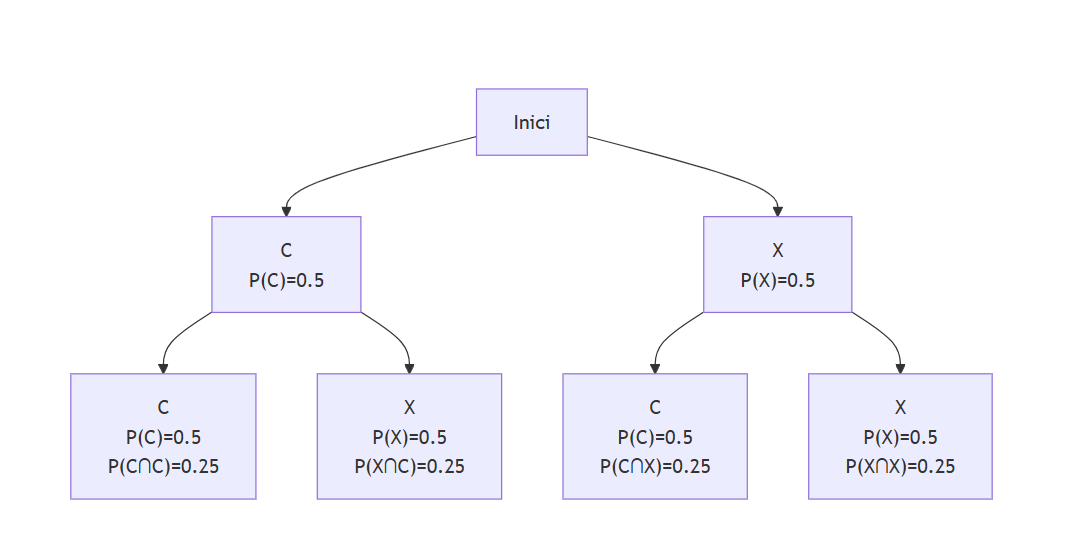
\includegraphics[width=0.6\textwidth]{da1.png}
\end{center}

Aquest és un exemple senzill, però els diagrames d’arbre poden ser molt més complexos, depenent de la quantitat d'esdeveniments i resultats possibles.
\end{exemple}

\begin{exercici} \noindent \textbf{Boles d’una bossa amb reposició}

Suposem que tenim una bossa amb 3 boles vermelles i 2 boles blaves. Si escollim una bola a l’atzar, la tornem a posar dins la bossa i després en seleccionem una altra, volem saber la probabilitat d’escollir una bola vermella primer i una bola blava després.

\begin{enumerate}
    \item \textbf{Dibuixar l’arbre:} Comença amb un punt des del qual es bifurquen dues branques: Vermella (V) i Blava (B). Des de la branca de Vermella, bifurca dues branques més per representar el resultat de la segona elecció: V-V i V-B. Fes el mateix per a la branca de Blava: B-V i B-B.
    \item \textbf{Assignar probabilitats:} La probabilitat d’escollir una bola Vermella en el primer intent és \(\frac{3}{5}\) i la de Blava és \(\frac{2}{5}\). Assigna aquestes probabilitats a les branques pertinents. Ja que estem tornant la bola a la bossa després d’escollir-la, les probabilitats no canvien per a la segona elecció.
    \item \textbf{Calcula la probabilitat d’interès:} Per determinar la probabilitat d’escollir V en la primera elecció i B en la segona, segueix la branca pertinent. La probabilitat serà:
    \[
    P(V \text{ i després } B) = \frac{3}{5} \times \frac{2}{5} = \frac{6}{25} = 0.24 \, (24\%).
    \]
\end{enumerate}

\begin{center}
      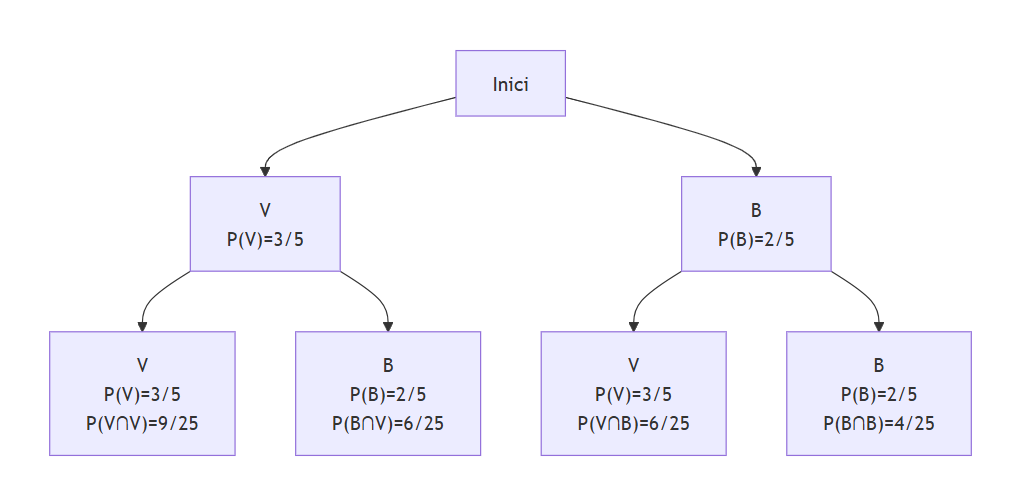
\includegraphics[width=0.7\textwidth]{da2.png}
\end{center}

Aquest exemple mostra com els diagrames d’arbre poden ser utilitzats en situacions on les probabilitats no són necessàriament iguals. També destaca la importància de tenir en compte les condicions del problema (en aquest cas, la reposició de la bola després d'escollir-la) quan es calculen probabilitats.

La probabilitat d’escollir una bola Vermella en la primera elecció i una bola Blava en la segona elecció és \(0.24\) o \(24\%\). Aquest exemple demostra com els diagrames d’arbre són útils per representar i calcular probabilitats en escenaris on els esdeveniments tenen probabilitats diferents.
\end{exercici}


\begin{exemple} \noindent \textbf{Sense reposició}

Si no tornem les boles a la bossa després d’escollir-les, les probabilitats canviaran per a la segona elecció. Vegem com afecta aquesta condició al nostre exemple.

\begin{enumerate}
    \item \textbf{Dibuixar l’arbre:} Igual que abans, comença amb un punt des del qual es bifurquen dues branques: Vermella (V) i Blava (B). Des de la branca de Vermella, bifurca dues branques més per representar el resultat de la segona elecció: V-V i V-B. Fes el mateix per a la branca de Blava: B-V i B-B.
    \item \textbf{Assignar probabilitats:} 
    \begin{itemize}
        \item La probabilitat de seleccionar una bola Vermella en el primer intent és \(\frac{3}{5}\), i la de Blava és \(\frac{2}{5}\). Assigna aquestes probabilitats a les branques pertinents.
        \item Si seleccionem una bola Vermella primer, queden 2 boles Vermelles i 2 boles Blaves a la bossa. Així que, per a la segona elecció:
        \[
        P(\text{Vermella}) = \frac{2}{4} = \frac{1}{2}, \quad P(\text{Blava}) = \frac{2}{4} = \frac{1}{2}.
        \]
        \item Si seleccionem una bola Blava primer, queden 3 boles Vermelles i 1 bola Blava a la bossa. Així que, per a la segona elecció:
        \[
        P(\text{Vermella}) = \frac{3}{4}, \quad P(\text{Blava}) = \frac{1}{4}.
        \]
    \end{itemize}
    \item \textbf{Calcula la probabilitat d’interès:} Per determinar la probabilitat d’escollir Vermella en la primera elecció i Blava en la segona (sense reposició), segueix la branca pertinent. La probabilitat serà:
    \[
    P(V \text{ i després } B) = \frac{3}{5} \times \frac{2}{4} = \frac{6}{20} = 0.3 \, (30\%).
    \]
\end{enumerate}

\begin{center}
       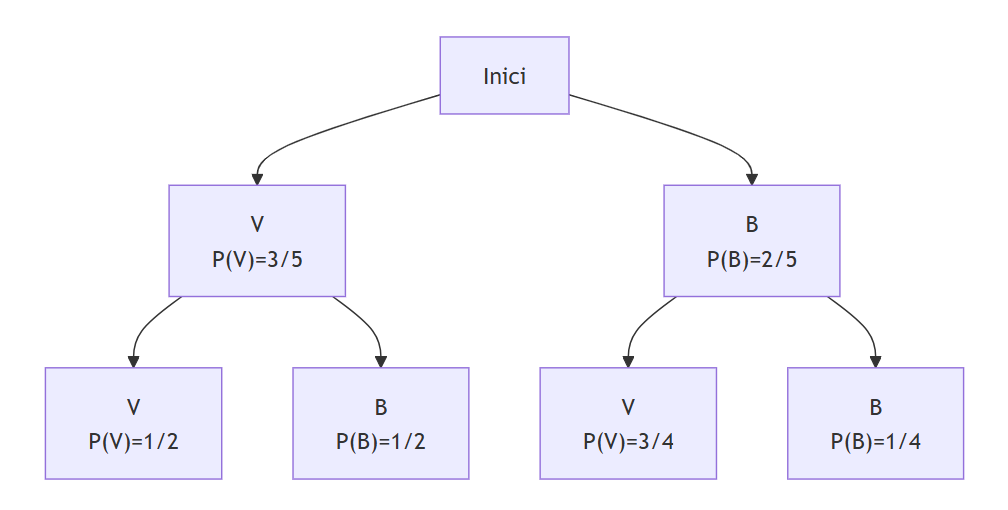
\includegraphics[width=0.7\textwidth]{da3.png}
\end{center}

La probabilitat d’escollir una bola Vermella en la primera elecció i una bola Blava en la segona elecció (sense reposició) és \(0.3\) o \(30\%\). Aquest resultat il·lustra com la falta de reposició pot afectar les probabilitats en escenaris successius. En aquest cas, la probabilitat ha augmentat lleugerament en comparació amb la situació amb reposició.
\end{exemple}

\subsection*{Exercicis}

\begin{exercici} [title=Exercici 1] \noindent  Una persona està considerant comprar un nou automòbil. Pot escollir entre un cotxe elèctric i un de gasolina. El 60$\%$ dels compradors prefereixen el cotxe elèctric, mentre que el 40$\%$ prefereixen el de gasolina. Dels que escullen el cotxe elèctric, el 70$\%$ volen un model petit i el 30$\%$ un model gran. Dels que escullen el model petit, el 50$\%$ volen color blanc i el 50$\%$ negre. Dels que escullen el model gran, el 60$\%$ volen color blanc i el 40$\%$ negre. Dels que escullen el cotxe de gasolina, el 80$\%$ volen un model esportiu i el 20$\%$ un model familiar. Dels que escullen el model esportiu, el 40$\%$ volen color vermell i el 60$\%$ blau. Dels que escullen el model familiar, el 70$\%$ volen color gris i el 30$\%$ verd.\\

    Resol els següents apartats utilitzant un diagrama d’arbre:
    
    \begin{enumerate}
        \item Quina és la probabilitat que un comprador esculli un cotxe elèctric, model petit i color blanc?
        \item Quina és la probabilitat que un comprador esculli un cotxe de gasolina, model esportiu i color blau?
    \end{enumerate}

    \begin{center}       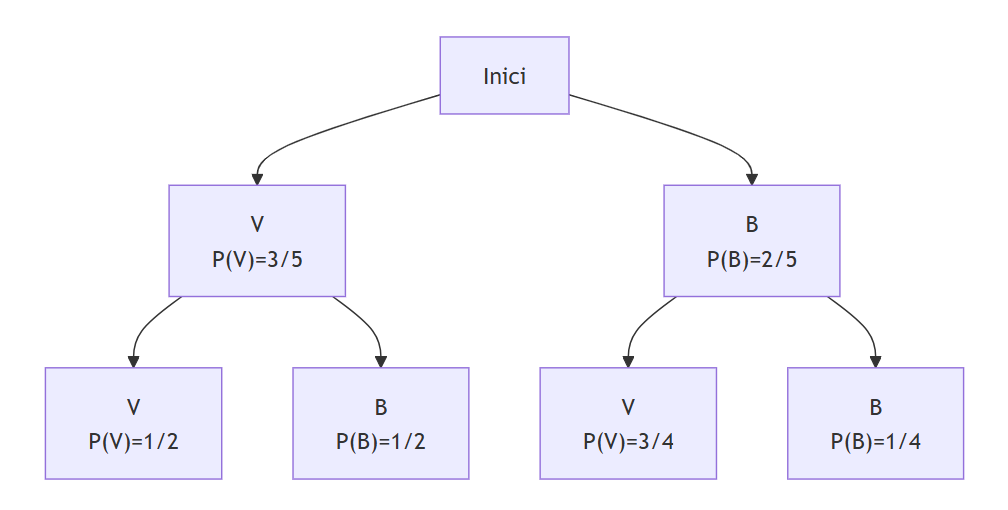
\includegraphics[width=0.55\textwidth]{da3.png}
    \end{center}

    \textbf{Pista:} Per resoldre aquests exercicis, multiplica les probabilitats corresponents a cada branca del diagrama d’arbre que condueixen a l’esdeveniment d’interès.
\end{exercici}

\begin{exercici} [title=Exercici 2]\noindent 
Una agència de viatges ofereix tres destinacions per a les vacances: muntanya, platja i ciutat. El 40\% dels clients escullen la muntanya, el 35\% la platja i el 25\% la ciutat. Dels que van a la muntanya, el 50\% decideixen fer senderisme, el 30\% esquí i el 20\% relaxar-se a un hotel. Dels que van a la platja, el 60\% decideixen practicar esports aquàtics, el 25\% prendre el sol i el 15\% fer excursions. Dels que van a la ciutat, el 70\% visiten museus, el 20\% fan compres i el 10\% assisteixen a concerts.

\begin{enumerate}
    \item Quina és la probabilitat que un client decideixi anar a la muntanya i fer senderisme?
    \item Quina és la probabilitat que un client decideixi anar a la platja i prendre el sol?
    \item Quina és la probabilitat que un client decideixi anar a la ciutat i assistir a concerts?
\end{enumerate}
\end{exercici}

\begin{exercici} [title=Exercici 3] \noindent 
En una ciutat, durant l'hivern, el 80\% dels dies són núvols. Dels dies núvols, el 50\% acaba plovent. Dels dies assolellats (20\% dels dies), només plou en un 10\%. Si un habitant decideix portar paraigua un dia a l'atzar:
\begin{enumerate}
    \item Quina és la probabilitat que sigui un dia núvol i plogui?
    \item Quina és la probabilitat que sigui un dia assolellat i no plogui?
\end{enumerate}
\end{exercici}

\begin{exercici} [title=Exercici 4] \noindent 
En una empresa, el 60\% dels empleats són homes i el 40\% són dones. Dels homes, el 70\% té un títol universitari, mentre que el 50\% de les dones té un títol universitari. Si se selecciona un empleat a l'atzar:
\begin{enumerate}
    \item Quina és la probabilitat que sigui un home amb un títol universitari?
    \item Quina és la probabilitat que sigui una dona sense títol universitari?
\end{enumerate}
\end{exercici}

\begin{exercici} [title=Exercici 5] \noindent 
Una pastisseria ven dos tipus de pastissos: xocolata i vainilla. El 70\% dels clients prefereixen el pastís de xocolata, mentre que el 30\% prefereixen el de vainilla. Dels clients que compren pastís de xocolata, el 60\% també compra una beguda. Dels clients que compren pastís de vainilla, el 80\% compra una beguda. Si un client entra a la pastisseria:
\begin{enumerate}
    \item Quina és la probabilitat que compri un pastís de xocolata i una beguda?
    \item Quina és la probabilitat que compri un pastís de vainilla però no una beguda?
\end{enumerate}
\end{exercici}

\section{Distribució Binomial}

\begin{concept} [title=Deficició] \noindent
La distribució binomial és una distribució de probabilitat discreta que descriu el nombre d'èxits en una seqüència fixa d'experiments independents de Bernoulli. Cada experiment té exactament dos resultats possibles, normalment denominats «èxit» i «fracàs».\\ 

Si designem per $p$ la probabilitat d'èxit en un sol assaig i per $q=1-p$; la probabilitat de fracàs, la funció de probabilitat d'una variable aleatòria $X$ que segueix una distribució binomial amb paràmetres $n$ i $p$ es dona per:

\[
P(X=k) = \binom{n}{k} p^k q^{n-k}
\]

on $k$ pot prendre valors entre $0$ i $n$.\\

\textbf{Paràmetres:}
\begin{itemize}
    \item $n$: Nombre total d'assajos independents. Valor enter no negatiu.
    \item $k$: Nombre d'èxits.
    \item $n-k$: Nombre de fracassos.
    \item $p$: Probabilitat d'èxit en un sol assaig. Aquest valor es troba en l'interval $[0,1]$.
    \item $\binom{n}{k}$ és el coeficient binomial, que representa el nombre de maneres de triar $k$ èxits d'un total de $n$ assajos.
\end{itemize}

La notació $\binom{n}{k}$, que sovint es llegeix com «$n$ sobre $k$», representa el coeficient binomial. Matemàticament, es calcula com:
\[
\binom{n}{k} = \frac{n!}{k!(n-k)!}
\]

Per exemple:
\[
\binom{5}{3} = \frac{5!}{3!(5-3)!} = 10
\]\\

Això indica que hi ha 10 maneres diferents de seleccionar 3 elements d'un conjunt de 5 elements sense tenir en compte l'ordre.
\end{concept}

\begin{exemple} \noindent 
Imaginem que llancem una moneda justa (no trucada) 5 vegades i volem saber quina és la probabilitat d'obtenir exactament 3 cares.

En aquest cas, $n=5$ (nombre de llançaments) i $p=0.5$ (probabilitat d'obtenir cara). Utilitzant la funció de massa de probabilitat:

\[
P(X=3) = \binom{5}{3} \cdot (0.5)^3 \cdot (1-0.5)^{5-3} = 0.3125
\]

La probabilitat és del $31.25\%$.
\end{exemple}

\begin{exemple} \noindent 
Una fàbrica produeix bombetes i, segons els seus controls de qualitat, el $2\%$ de les bombetes són defectuoses. Si agafem una mostra aleatòria de 100 bombetes, quina és la probabilitat que exactament 3 bombetes siguin defectuoses?

Aquí, $n=100$ (nombre de bombetes) i $p=0.02$ (probabilitat que una bombeta sigui defectuosa). Aplicant la fórmula de la distribució binomial:

\[
P(X=3) = \binom{100}{3} \cdot (0.02)^3 \cdot (1-0.02)^{100-3}
\]

Després de fer els càlculs, obtenim $P(X=3) \approx 0.1823$, és a dir, un $18.23\%$.
\end{exemple}

\begin{exemple} \noindent 
Una empresa llança una campanya de màrqueting per correu electrònic. La probabilitat que un client compri després de rebre el correu és del $10\%$. Si l'empresa envia correus a 20 clients diferents, quina és la probabilitat d'aconseguir exactament 4 vendes?

En aquest cas, $n=20$ i $p=0.1$. La probabilitat es calcula com:

\[
P(X=4) = \binom{20}{4} \cdot (0.1)^4 \cdot (1-0.1)^{20-4}
\]

El resultat és aproximadament $P(X=4) \approx 0.0881$, o un $8.81\%$.
\end{exemple}

\begin{exercici}[title=Exercicis proposats] \noindent 
\begin{enumerate}
    \item \textbf{Moneda trucada:} Una moneda no és justa, i la probabilitat d'obtenir cara és $0.6$. Si es llança 10 vegades, quina és la probabilitat d'obtenir exactament 6 cares?
    \item \textbf{Examen tipus test:} En un examen tipus test amb 20 preguntes de resposta múltiple, cada pregunta té 4 opcions (només una correcta). Si un estudiant respon al atzar, quina és la probabilitat que encerti exactament 5 preguntes?
    \item \textbf{Taxa natalitat:} Un hospital registra una taxa de natalitat de $52\%$ per a nens i $48\%$ per a nenes. Si en un dia neixen 15 nadons, quina és la probabilitat que exactament 8 siguin nens?
\end{enumerate}
\end{exercici}

\begin{exercici} [title=]  \noindent  
\begin{enumerate}[start=4]
    \item \textbf{Competició de Futbol:}  
    En una lliga de futbol, un equip té una probabilitat del $60\%$ de guanyar qualsevol partit. Si juguen 3 partits, quina és la probabilitat que guanyin exactament 2?

    \item \textbf{Producció de Galetes:}  
    Una fàbrica de galetes té un $5\%$ de probabilitat de produir una galeta trencada. Si es produeixen 4 galetes, quina és la probabilitat que no hi hagi cap galeta trencada?


\end{enumerate}
\end{exercici}

\begin{exercici}[title=Exercicis proposats amb solucions] \noindent 
\begin{enumerate}
    \item \textbf{Tirades de Dau:}  
    Si tires un dau just 6 vegades, quina és la probabilitat que surti el número 5 exactament 2 vegades?  
    \fbox{Solució: $20.09\%$}

    \item \textbf{Averies de Cotxe:}  
    Si la probabilitat que un cotxe tingui una avaria en un mes és del $10\%$, quina és la probabilitat que tingui almenys 1 avaria en 3 mesos?  
    \fbox{Solució: $27.10\%$}

    \item \textbf{Pluja:}  
    Si la probabilitat que plogui un dia qualsevol és del $30\%$, quina és la probabilitat que no plogui en 5 dies consecutius?  
    \fbox{Solució: $0.24\%$}

    \item \textbf{Producció d'Ordinadors:}  
    Una fàbrica té una probabilitat del $2\%$ de produir un ordinador defectuós. Si produeixen 50 ordinadors, quina és la probabilitat que almenys 3 d'ells siguin defectuosos?  
    \fbox{Solució: $7.84\%$}

    \item \textbf{Examen de Matemàtiques:}  
    En un examen de matemàtiques amb 10 preguntes, un estudiant té una probabilitat del $80\%$ d'encertar cada pregunta. Quina és la probabilitat que l'estudiant encerti com a mínim 8 preguntes?  
    \fbox{Solució: $67.78\%$}

    \item \textbf{Competició de Natació:}  
    En una competició de natació, un nadador té una probabilitat del $75\%$ de guanyar una cursa. Si competeix en 4 curses, quina és la probabilitat que guanyi totes elles?  
    \fbox{Solució: $31.64\%$}

    \item \textbf{Cultiu de Roses:}  
    Un jardiner té una probabilitat del $85\%$ que una rosa plantada creixi amb èxit. Si planta 7 roses, quina és la probabilitat que almenys 6 d'elles creixin amb èxit?  
    \fbox{Solució: $71.66\%$}

    \item \textbf{Venda de Productes:}  
    Un comercial té una probabilitat del $50\%$ de tancar una venda quan es reuneix amb un client. Si es reuneix amb 6 clients en un dia, quina és la probabilitat que tanqui com a mínim 4 vendes?  
    \fbox{Solució: $34.38\%$}

    \item \textbf{Recepció de Correus:}  
    Si la probabilitat que un empleat rebi un correu important en un dia qualsevol és del $20\%$, quina és la probabilitat que rebi exactament 2 correus importants en una setmana de 5 dies?  
    \fbox{Solució: $20.48\%$}

    \item \textbf{Producció de Xocolata:}  
    Una fàbrica de xocolata té un $1\%$ de probabilitat de produir una barra de xocolata amb un embolcall defectuós. Si produeixen 100 barres, quina és la probabilitat que hi hagi exactament 1 amb un embolcall defectuós?  
    \fbox{Solució: $36.97\%$}
\end{enumerate}
\end{exercici}

\section{Distribució Normal}

\begin{concept}[title=Definició i Propietats] \noindent La distribució normal, també coneguda com a distribució gaussiana, és una de les distribucions de probabilitat contínues més conegudes i utilitzades en estadística. \\

La seva funció de densitat de probabilitat (fdp) té forma de campana de Gauss i està definida per dos paràmetres: la mitjana ($\mu$) i la desviació estàndard ($\sigma$).\\

La fórmula matemàtica de la fdp és:
\[
f(x) = \frac{1}{\sigma \sqrt{2\pi}} e^{-\frac{1}{2} \left(\frac{x-\mu}{\sigma}\right)^2}
\]

\begin{center}
    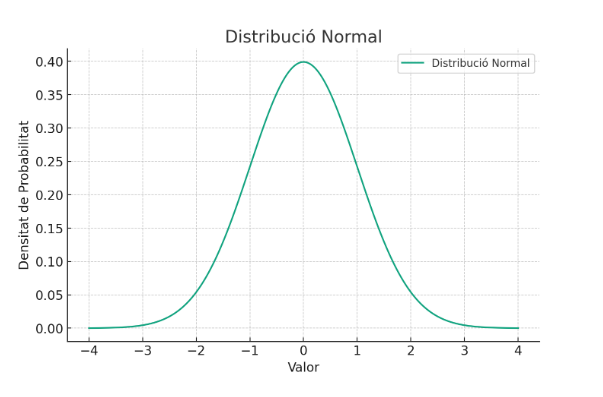
\includegraphics[width=0.7\textwidth]{dn1.png}
\end{center}

Propietats principals:
\begin{itemize}
    \item És simètrica respecte a la seva mitjana $\mu$.
    \item L'àrea sota la corba (probabilitat total) és 1.
    \item Aproximadament el 68\% de les dades estan dins d'1 desviació estàndard, el 95\% dins de 2, i el 99.7\% dins de 3.
\end{itemize}
\end{concept}

\begin{concept}[title=Paràmetres] \noindent Els paràmetres que defineixen una distribució nomral són:
\begin{itemize}
    \item $\mu$: La mitjana indica on es troba el pic de la corba.
    \item $\sigma$: La desviació estàndard mesura la dispersió respecte a la mitjana.
    \item $\sigma^2$: És la variància, el quadrat de la desviació estàndard.
\end{itemize}
\end{concept}

\begin{concept}[title=Funció de Densitat de Probabilitat] \noindent La funció de densitat de probabilitat (fdp) descriu la probabilitat que una variable aleatòria $X$ prengui un valor específic $x$. \\

La seva fórmula és:
\[
f(x) = \frac{1}{\sigma \sqrt{2\pi}} e^{-\frac{1}{2} \left(\frac{x-\mu}{\sigma}\right)^2}
\]
Com que és una distribució contínua, la probabilitat d'un valor puntual és 0; en canvi, es calculen probabilitats d'interval.\\

L'àrea de la regió tancada entre $f(x), OX$ i les rectes $x=a$ i $x=b$ és la probabilitat que la variable $X$ estigui en l'interval $[a, b]$.\\
\begin{center}

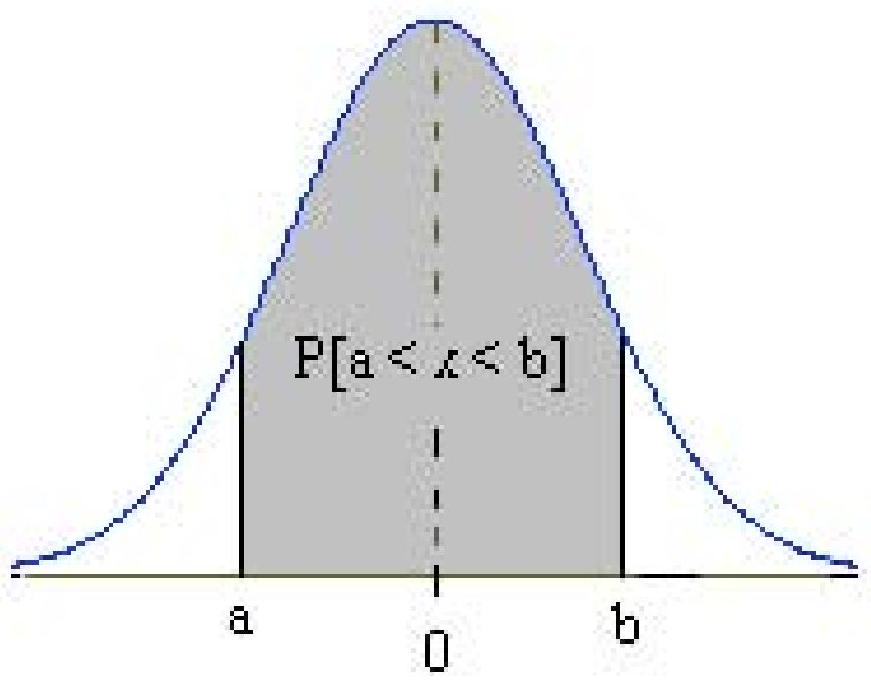
\includegraphics[scale=0.15]{2025_04_16_212c3443f91efdb33a77g-2.jpg}
    
\end{center}

\end{concept}

\begin{exemple} \noindent Alçades d'Adults
Suposa que l'alçada d'adults en una població segueix una distribució normal amb $\mu = 170$ cm i $\sigma = 10$ cm.\\

1. Visualització: La funció de densitat de probabilitat per aquesta distribució és una corba de campana centrada a 170 cm.
\begin{center}
    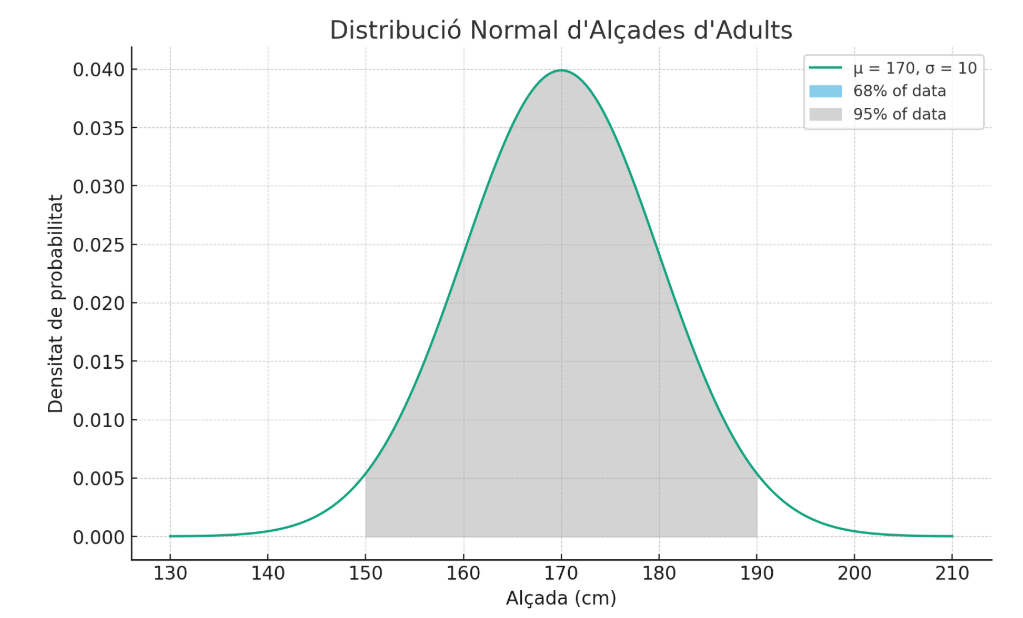
\includegraphics[width=0.7\textwidth]{dn2.png}
\end{center}
\end{exemple}

\subsection*{Distribució Normal Estàndard i Estandardització}
\begin{concept}[title=Definició] \noindent
La distribució normal estandarditzada $N(0,1)$ té una mitjana de 0 i una desviació estàndard d'1.\\

\begin{center}
    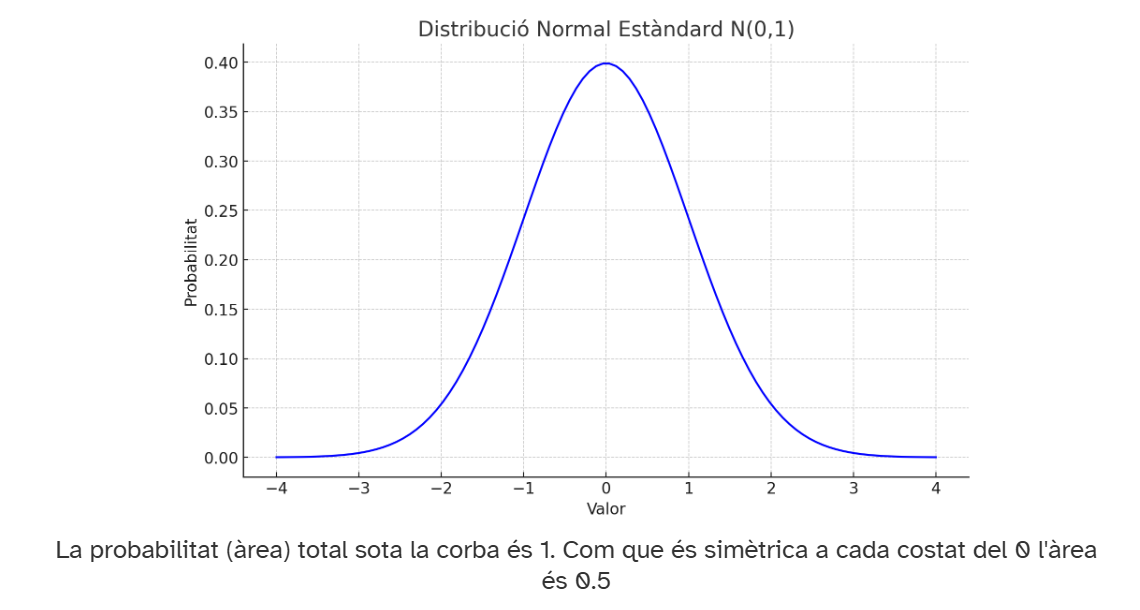
\includegraphics[width=0.7\textwidth]{dn3.png}
\end{center}

Per convertir qualsevol distribució $N(\mu, \sigma)$ a $N(0,1)$, s'utilitza la fórmula d'estandardització:
\[
Z = \frac{X - \mu}{\sigma}
\]
On $Z$ és la variable estandarditzada.\\ 

Aquest procés permet utilitzar la taula de distribució normal estàndard per calcular probabilitats.


$$
P[x \leq X ]=P[Z\leq \frac{X-\mu}{\sigma}]
$$

El canvi $x \rightarrow \dfrac{x-\mu}{\sigma}=Z\;$   s'anomena tipificació de la variable.\\

La variable tipificada $Z$ segueix una distribució $N(0,1)$\\

\textbf{Exemple}: En una $N(6,4)$, calcular $P[x<3]$

$$
P[x<3]=P\left[z<\frac{3-6}{4}\right]=P[z<-0,75]=1-P[z<0,75]=1-0,7734=0,2266
$$


\end{concept}

\subsection*{Ús de la taula $N(0,1)$ i Càlcul de Probabilitats}
\begin{concept}[title=Ús de la taula] \noindent
En la distribució de la $N(0,1)$, a la variable se sol representar per la lletra $Z$. \\

La taula amb la qual treballarem ens dóna les probabilitats $P[z \leq k]$ per a valors de $k$ de 0 a 4 centèsimes. A aquestes probabilitats se les anomena $F(k)$:

$$
F(k)=P[x \leq k] \text { z es distribueix segons una } N(0,1)
$$\\

$F(k)$ és, doncs, la funció de distribució d'aquesta variable aleatòria.\\

\begin{center}
   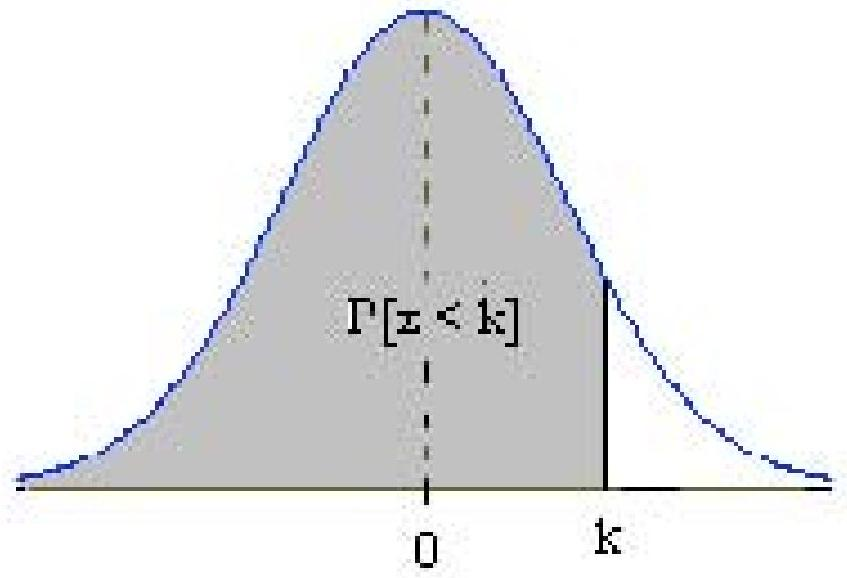
\includegraphics[scale=0.15]{2025_04_16_212c3443f91efdb33a77g-2(1)} 
\end{center}


El valor de $k$ es busca de la següent manera:

\begin{itemize}
  \item Unitats i dècimes a la columna de l'esquerra.
  \item Centèsimes a la fila de dalt.
  \item El número que ens dóna la taula és el valor de: $F(k)=P[z \leq k]$.
\end{itemize}

\textbf{Exemples}:

\begin{itemize}
  \item $P[z \leq 0,45]=F(0,45)=0,6736$
  \item $P[z \leq 1,2]=F(1,2)=0,8849$
  \item $P[z \leq 1]=F(1)=0,8413$
\end{itemize}

Recíprocament, si coneixem el valor de la probabilitat $P[z \leq k]$, es pot saber el valor de $k$. Exemples:

\begin{itemize}
  \item $P[z \leq k]=F(k)=0,7190 \Rightarrow k=0,58$
  \item $P[z \leq k]=F(k)=0,8643 \Rightarrow k=1,1$
  \item $P[z \leq k]=F(k)=0,5560 \Rightarrow k=0,14$
\end{itemize}

Recordem que en la distribució de variable contínua les probabilitats puntuals són nul·les, $P[x=k]=0$. Per tant, $P[x \leq k]=P[z<k]$
\end{concept}

\begin{concept}[title=Càlcul de probabilitats] \noindent Als exercicis podem trobar-nos diferents casuístiques:

\begin{itemize}
  \item Si $k \geq 0$, les probabilitats $P[z \leq k]=P[z<k]$ es troben directament a la taula.
  
  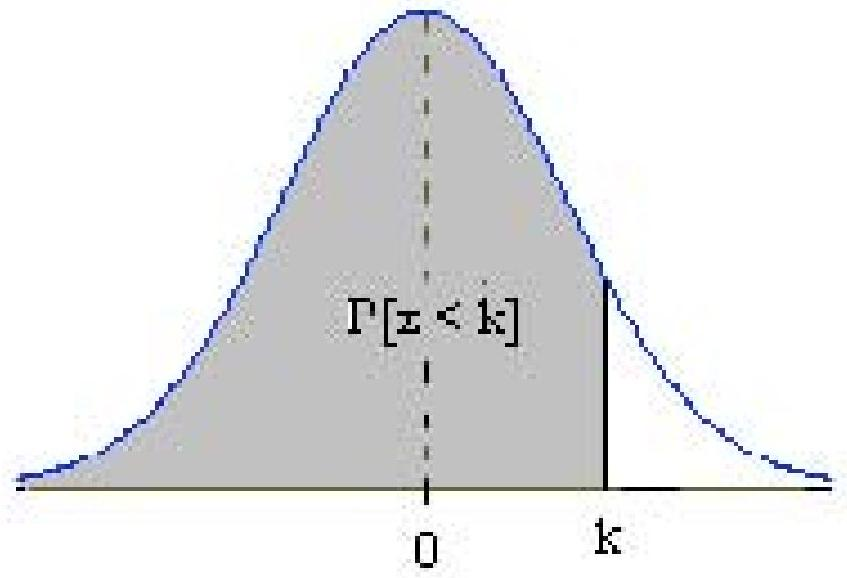
\includegraphics[scale=0.12,]{2025_04_16_212c3443f91efdb33a77g-2(1)}\\
  
  \item Si $k \geq 0, P[z \geq k]=1-P[z \leq k]$\\
  
  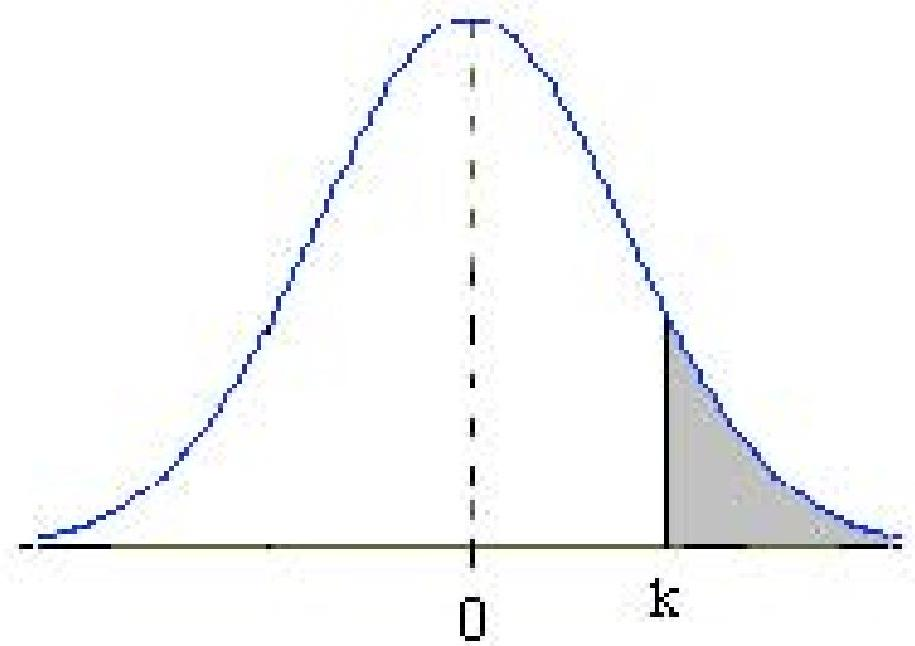
\includegraphics[scale=0.1]{2025_04_16_212c3443f91efdb33a77g-3}
  
Exemple: $
P[z \geq 1,73]=1-P[z \leq 1,73]=1-0,9582=0,0418
$\\

  \item Si $k<0, P[z \leq k]=P[z \geq-k]=1-P[z \leq-k]$\\

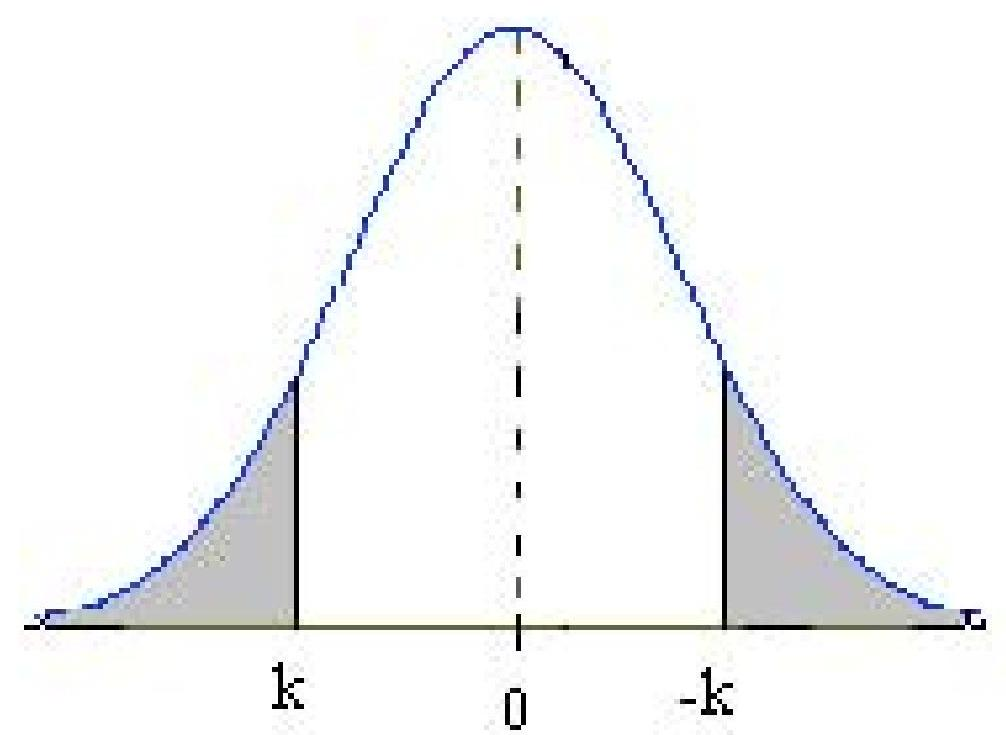
\includegraphics[scale=0.1]{2025_04_16_212c3443f91efdb33a77g-4(1)}

Exemple:
$
P[z \leq-0,83]=P[z \geq 0,83]=1-P[z \leq 0,83]=1-0,7967=0,2033
$\\

  \item Si $k<0, P[z \geq k]=P[z \leq-k]$\\
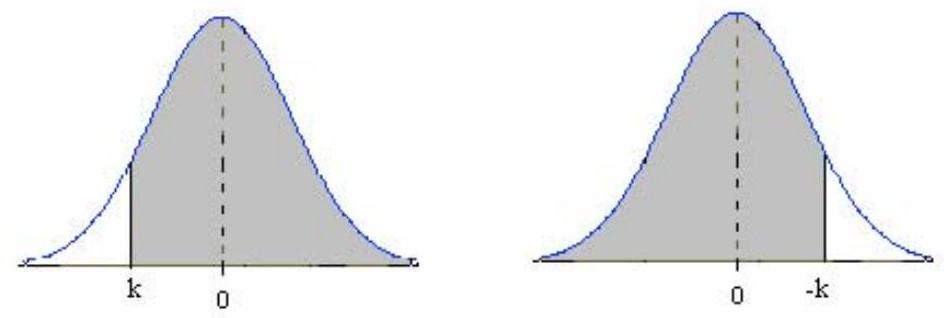
\includegraphics[scale=0.2]{2025_04_16_212c3443f91efdb33a77g-4}

Exemple:
$
P[z \leq-0,83]=P[z \geq 0,83]=1-P[z \leq 0,83]=-0,7967=0,2033
$\\
  \item $P[a \leq z \leq b]=P[z \leq b]-P[z \leq z]$\\
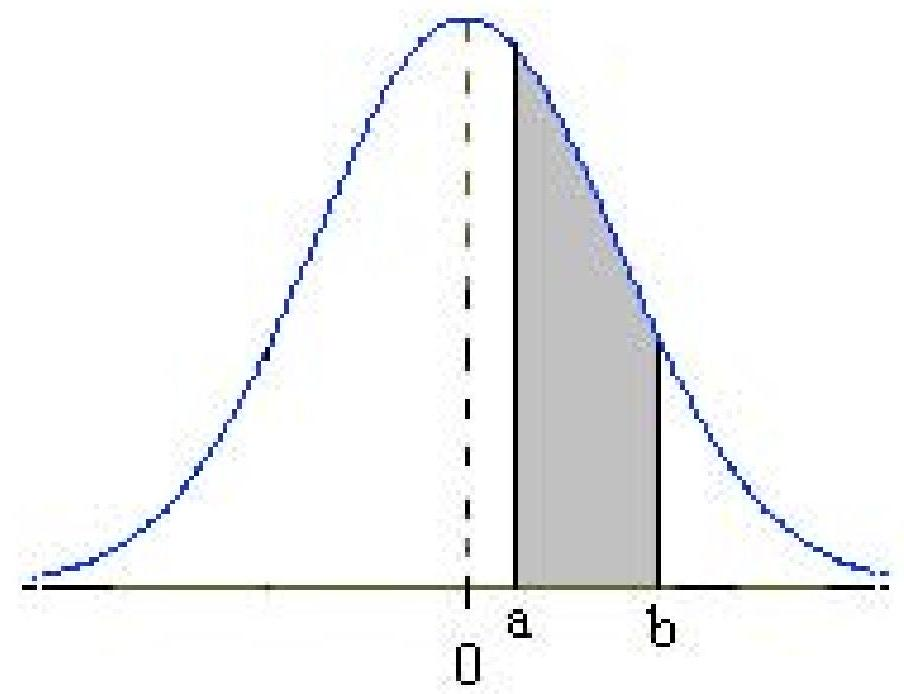
\includegraphics[scale=0.1]{2025_04_16_212c3443f91efdb33a77g-5}

Exemple: $
P[0,21 \leq z \leq 1,34]=P[z \leq 1,34]-P[z \leq 0,21]=0,9099-0,5832=0,3267
$
\end{itemize}
  
\end{concept}

\begin{exemple}

\begin{enumerate}
    \item L'alçada dels alumnes d'un col·legi segueix una distribució normal amb una mitjana de 170 cm i una desviació estàndard de 15 cm. Quina és la probabilitat que un alumne triat a l'atzar tingui una alçada inferior a 190 cm?
    
    \textbf{Solució:} La probabilitat que un alumne tingui una alçada inferior a 190 cm és aproximadament del 90.88\%.
    
    \[
    P(X < 190) = P\left(Z< \frac{190 - 170}{15} \right) = P(Z< 1.33) \approx 0.9088
    \]

    \item El temps per completar un examen final segueix una distribució normal amb una mitjana de 120 minuts i una desviació estàndard de 20 minuts. Quina és la probabilitat que un estudiant acabi l'examen en menys de 150 minuts?
    
    \textbf{Solució:} La probabilitat que un estudiant acabi l'examen en menys de 150 minuts és aproximadament del 93.32\%.
    
    \[
    P(X < 150) = P\left(Z< \frac{150 - 120}{20} \right) = P(Z< 1.5) \approx 0.9332
    \]


    \item El consum de combustible (en litres per cada 100 km) de vehicles d'un cert model segueix una distribució normal amb una mitjana de 8 litres i una desviació estàndard d'1 litre. Quina és la probabilitat que un vehicle d'aquest model consuma menys de 9.5 litres per cada 100 km?
    
    \textbf{Solució:} La probabilitat que un vehicle consuma menys de 9.5 litres per cada 100 km és aproximadament del 93.32\%.
    
    \[
    P(X < 9.5) = P\left(Z< \frac{9.5 - 8}{1} \right) = P(Z< 1.5) \approx 0.9332
    \]

    \item En una ciutat, la temperatura mitjana durant l'any segueix una distribució normal amb una mitjana de 15°C i una desviació estàndard de 5°C. Quina és la probabilitat que en un dia qualsevol la temperatura sigui inferior a 21°C?
    
    \textbf{Solució:} La probabilitat que la temperatura sigui inferior a 21°C un dia qualsevol és aproximadament del 88.49\%.
    \[
    P(X < 21) = P\left(Z< \frac{21 - 15}{5} \right) = P(Z< 1.2) \approx 0.8849
    \]

    \item La durada de les trucades telefòniques en un centre d'atenció al client segueix una distribució normal amb una mitjana de 4 minuts i una desviació estàndard d'1 minut. Quina és la probabilitat que una trucada seleccionada a l'atzar tingui una durada inferior a 5.5 minuts?
    
    \textbf{Solució:} La probabilitat que una trucada tingui una durada inferior a 5.5 minuts és aproximadament del 93.32\%.
    
    \[
    P(X < 5.5) = P\left(Z< \frac{5.5 - 4}{1} \right) = P(Z< 1.5) \approx 0.9332
    \]
\end{enumerate}
\end{exemple}

\begin{exemple}[title=]
    
\begin{enumerate}[start=6]

   \item Les puntuacions obtingudes pels jugadors en un videojoc popular segueixen una distribució normal amb una mitjana de 500 punts i una desviació estàndard de 100 punts. Quina és la probabilitat que un jugador seleccionat a l'atzar obtingui una puntuació inferior a 453 punts?
    
    \textbf{Solució:} La probabilitat que un jugador obtingui una puntuació inferior a 453 punts és del 31.92\%.
    
    \[
    P(X < 453) = P\left(Z< \frac{453 - 500}{100} \right) = P(Z< -0.47) = 1 - P(Z< 0.47) \approx 0.3192
    \]

    \item Les temperatures matinals en una ciutat durant l'hivern segueixen una distribució normal amb una mitjana de 5ºC i una desviació estàndard de 3ºC. Quina és la probabilitat que en un dia a l'atzar la temperatura matinal sigui inferior a 0ºC?
    
    \textbf{Solució:} La probabilitat que la temperatura matinal sigui inferior a 0ºC és del 4.78\%.
    
    \[
    P(X < 0) = P\left(Z< \frac{0 - 5}{3} \right) = P(Z< -1.67) = 1 - P(Z< 1.67) \approx 0.0478
    \]

    \item La velocitat de tipus dels participants en un concurs de mecanografia segueix una distribució normal amb una mitjana de 60 paraules per minut i una desviació estàndard de 10 paraules per minut. Quina és la probabilitat que un participant triat a l'atzar tingui una velocitat de tipus inferior a 43 paraules per minut?
    
    \textbf{Solució:} La probabilitat que un participant tingui una velocitat de tipus inferior a 43 paraules per minut és del 4.46\%.
    
    \[
    P(X < 43) = P\left(Z< \frac{43 - 60}{10} \right) = P(Z< -1.7) = 1 - P(Z< 1.7) \approx 0.0446
    \]

    \item El pes de les maletes facturades en un aeroport segueix una distribució normal amb una mitjana de 23 kg i una desviació estàndard de 5 kg. Quina és la probabilitat que una maleta triada a l'atzar pesi menys de 14 kg?
    
    \textbf{Solució:} La probabilitat que una maleta pesi menys de 14 kg és del 3.59\%.
    
    \[
    P(X < 14) = P\left(Z< \frac{14 - 23}{5} \right) = P(Z< -1.8) = 1 - P(Z< 1.8) \approx 0.0359
    \]
\end{enumerate}
    
\end{exemple}

\begin{exemple} [title=]

\begin{enumerate} [start=10]

    \item La durada de les trucades telefòniques en una companyia segueix una distribució normal amb una mitjana de 4 minuts i una desviació estàndard d'1 minut. Quina és la probabilitat que una trucada seleccionada a l'atzar tingui una durada inferior a 2 minuts i mig?
    
    \textbf{Solució:} La probabilitat que una trucada tingui una durada inferior a 2 minuts i mig és del 6.68\%.
    
    \[
    P(X < 2.5) = P\left(Z< \frac{2.5 - 4}{1} \right) = P(Z< -1.5) = 1 - P(Z< 1.5) \approx 0.0668
    \]

    \item En un examen, les puntuacions segueixen una distribució normal amb una mitjana de 70 punts i una desviació estàndard de 10 punts. Quina és la probabilitat que un estudiant triat a l'atzar obtingui més de 80 punts?
    
    \textbf{Solució:} La probabilitat que un estudiant obtingui més de 80 punts és del 15.87\%.
    
    \[
    P(X > 80) = 1 - P\left(Z< \frac{80 - 70}{10} \right) = 1 - P(Z< 1) \approx 0.1587
    \]

    \item Les temperatures diürnes d'una ciutat durant l'estiu segueixen una distribució normal amb una mitjana de 28ºC i una desviació estàndard de 4ºC. Quina és la probabilitat que la temperatura en un dia qualsevol superi els 33ºC?
    
    \textbf{Solució:} La probabilitat que la temperatura superi els 33ºC és del 10.56\%.
    
    \[
    P(X > 33) = 1 - P\left(Z< \frac{33 - 28}{4} \right) = 1 - P(Z< 1.25) \approx 0.1056
    \]

    \item La velocitat de descàrrega d'una connexió a internet en una ciutat segueix una distribució normal amb una mitjana de 50 Mbps i una desviació estàndard de 5 Mbps. Quina és la probabilitat que, en una comprovació aleatòria, la velocitat de descàrrega superi els 60 Mbps?
    
    \textbf{Solució:} La probabilitat que la velocitat de descàrrega superi els 60 Mbps és del 2.28\%.
    
    \[
    P(X > 60) = 1 - P\left(Z< \frac{60 - 50}{5} \right) = 1 - P(Z< 2) \approx 0.0228
    \]

    \item En un camp d'experimentació agrícola, l'altura de cert tipus de plantes segueix una distribució normal amb una mitjana de 120 cm i una desviació estàndard de 15 cm. Quina és la probabilitat que una planta triada a l'atzar tingui una altura superior a 135 cm?
    
    \textbf{Solució:} La probabilitat que una planta tingui una altura superior a 135 cm és del 15.87\%.
    
    \[
    P(X > 135) = 1 - P\left(Z< \frac{135 - 120}{15} \right) = 1 - P(Z< 1) \approx 0.1587
    \]
\end{enumerate}
    
\end{exemple}

\begin{exemple} [title=]

\begin{enumerate} [start=15]

    \item El consum de combustible d'un model específic de cotxe segueix una distribució normal amb una mitjana de 8 litres per cada 100 km i una desviació estàndard d'1 litre. Quina és la probabilitat que, en un trajecte aleatori, el consum de combustible d'aquest model de cotxe superi els 9 litres per cada 100 km?
    
    \textbf{Solució:} La probabilitat que el consum de combustible superi els 9 litres per cada 100 km és del 15.87\%.
    
    \[
    P(X > 9) = 1 - P\left(Z< \frac{9 - 8}{1} \right) = 1 - P(Z< 1) \approx 0.1587
    \]

    \item En una empresa de tecnologia, els salaris segueixen una distribució normal amb una mitjana de 3000 euros i una desviació estàndard de 500 euros. Quina és la probabilitat que el salari d'un treballador seleccionat a l'atzar estigui entre 2600 i 3410 euros?
    
    \textbf{Solució:} La probabilitat que el salari d'un treballador estigui entre 2600 i 3410 euros és del 58.20\%.
    
    \begin{align*}
    P(2600 < X < 3410) &= P\left(Z< \frac{3410 - 3000}{500} \right) - P\left(Z< \frac{2600 - 3000}{500} \right) \\
    &= P(Z< 0.82) - P(Z< -0.8) \approx 0.5820
    \end{align*}

    \item Els resultats de colesterol en sang en una població segueixen una distribució normal amb una mitjana de 200 mg/dL i una desviació estàndard de 30 mg/dL. Quina és la probabilitat que una persona tingui un resultat de colesterol entre 185 i 220 mg/dL?
    
    \textbf{Solució:} La probabilitat que una persona tingui un resultat de colesterol entre 185 i 220 mg/dL és del 43.90\%.
    
    \begin{align*}
    P(185 < X < 220) &= P\left(Z< \frac{220 - 200}{30} \right) - P\left(Z< \frac{185 - 200}{30} \right) \\
    &= P(Z< 0.67) - P(Z< -0.5) \approx 0.4390
    \end{align*}


    \item En una marató, els temps de finalització segueixen una distribució normal amb una mitjana de 4 hores i una desviació estàndard de 0.5 hores. Quina és la probabilitat que un corredor acabi entre 3 i 4.25 hores?
    
    \textbf{Solució:} La probabilitat que un corredor acabi entre 3 i 4.25 hores és del 66.87\%.
    
    \begin{align*}
    P(3 < X < 4.25) &= P\left(Z< \frac{4.25 - 4}{0.5} \right) - P\left(Z< \frac{3 - 4}{0.5} \right) \\
    &= P(Z< 0.5) - P(Z< -2) \approx 0.6687  
    \end{align*}
\end{enumerate}
    
\end{exemple}

\begin{exemple} [title=]

\begin{enumerate} [start=19]

    \item El pes dels paquets enviats per una empresa de missatgeria segueix una distribució normal amb una mitjana de 5 kg i una desviació estàndard d'1 kg. Quina és la probabilitat que un paquet seleccionat a l'atzar tingui un pes entre 4.35 i 5.5 kg?
    
    \textbf{Solució:} La probabilitat que un paquet tingui un pes entre 4.35 i 5.5 kg és del 43.36\%.
    
    \begin{align*}
    P(4.35 < X < 5.5) &= P\left(Z< \frac{5.5 - 5}{1} \right) - P\left(Z< \frac{4.35 - 5}{1} \right) \\
    &= P(Z< 0.5) - P(Z< -0.65) \approx 0.4336  
    \end{align*}

    

    \item El consum d'electricitat mensual en les llars segueix una distribució normal amb una mitjana de 300 kWh i una desviació estàndard de 50 kWh. Quina és la probabilitat que el consum d'una llar en un mes estigui entre 270 i 325 kWh?
    
    \textbf{Solució:} La probabilitat que el consum d'una llar en un mes estigui entre 270 i 325 kWh és del 41.72\%.
    
    \begin{align*}
    P(270 < X < 325) &= P\left(Z< \frac{325 - 300}{50} \right) - P\left(Z< \frac{270 - 300}{50} \right) \\
    &= P(Z< 0.5) - P(Z< -0.6) \approx 0.4172
    \end{align*}


    \item Pes dels paquets de cafè: Una fàbrica empaqueta cafè en bosses de 500 grams. Suposa que el pes dels paquets segueix una distribució normal amb una mitjana de 500 grams i una desviació estàndard de 10 grams. Quina és la probabilitat que un paquet seleccionat a l'atzar pesi entre 485 i 515 grams?
    
    \textbf{Solució:} La probabilitat que un paquet de cafè pesi entre 485 i 515 grams és del 86.64\%.
    
    \begin{align*}
    P(485 < X < 515) &= P\left(Z< \frac{515 - 500}{10} \right) - P\left(Z< \frac{485 - 500}{10} \right) \\
    &= P(Z< 1.5) - P(Z< -1.5) \approx 0.8664
    \end{align*}


    \item Resultats d'una prova: Els resultats d'una prova estandarditzada distribuïda entre tots els estudiants de secundària tenen una mitjana de 50 i una desviació estàndard de 10. Quina és la probabilitat que un estudiant seleccionat a l'atzar obtingui una puntuació superior a 65?
    
    \textbf{Solució:} La probabilitat que un estudiant obtingui una puntuació superior a 65 és del 6.68\%.
    
    \[
    P(X > 65) = 1 - P\left(Z< \frac{65 - 50}{10} \right) = 1 - P(Z< 1.5) \approx 0.0668
    \]
\end{enumerate}
\end{exemple}

\begin{exemple} [title=]

\begin{enumerate} [start=23]

    \item Vida útil d'una bombeta: La vida útil d'una bombeta produeix per una companyia es distribueix normalment amb una mitjana de 1200 hores i una desviació estàndard de 100 hores. Quina és la probabilitat que una bombeta duri més de 1400 hores?
    
    \textbf{Solució:} La probabilitat que una bombeta duri més de 1400 hores és del 2.28\%.
    
    \[
    P(X > 1400) = 1 - P\left(Z< \frac{1400 - 1200}{100} \right) = 1 - P(Z< 2) \approx 0.0228
    \]

    \item Suposa que l'alçada dels adults d'un país està distribuïda seguint una normal amb una mitjana de 170 cm i una desviació estàndard de 7 cm. Quina és la probabilitat que una persona seleccionada a l'atzar tingui una alçada inferior a 160 cm?
    
    \textbf{Solució:} La probabilitat que una persona tingui una alçada inferior a 160 cm és del 7.66\%.
    
    \[
    P(X < 160) = P\left(Z< \frac{160 - 170}{7} \right) = P(Z< -1.43) = 1 - P(Z< 1.43) \approx 0.0766
    \]

    \item Consum de combustible: El consum de combustible d'un cert model de cotxe segueix una distribució normal amb una mitjana de 15 km/l i una desviació estàndard de 2 km/l. Si un conductor selecciona a l'atzar un cotxe d'aquest model, quina és la probabilitat que el cotxe tingui un consum entre 13 km/l i 18 km/l?
    
    \textbf{Solució:} La probabilitat que un cotxe tingui un consum entre 13 km/l i 18 km/l és del 77.45\%.
    
    \begin{align*}
    P(13 < X < 18) &= P\left(Z< \frac{18 - 15}{2} \right) - P\left(Z< \frac{13 - 15}{2} \right) \\
    &= P(Z< 1.5) - P(Z< -1) \approx 0.7745 
    \end{align*}


    \item Durada de les trucades: Les trucades a un centre d'atenció al client d'una companyia de telefonia tenen una durada mitjana de 8 minuts amb una desviació estàndard de 2 minuts. Quina és la probabilitat que una trucada seleccionada a l'atzar duri menys de 5 minuts?
    
    \textbf{Solució:} La probabilitat que una trucada duri menys de 5 minuts és del 6.68\%.
    
    \[
    P(X < 5) = P\left(Z< \frac{5 - 8}{2} \right) = P(Z< -1.5) = 1 - P(Z< 1.5) \approx 0.0668
    \]

    \item Pes dels fruits: El pes d'unes pomes d'una certa varietat es distribueix normalment amb una mitjana de 150 grams i una desviació estàndard de 20 grams. Si compres una poma a l'atzar, quina és la probabilitat que pesi més de 180 grams?
    
    \textbf{Solució:} La probabilitat que una poma pesi més de 180 grams és del 6.68\%.
    
    \[
    P(X > 180) = 1 - P\left(Z< \frac{180 - 150}{20} \right) = 1 - P(Z< 1.5) \approx 0.0668
    \]
\end{enumerate}
\end{exemple}

\begin{exemple} [title=]

\begin{enumerate}[start=28]

    \item Temps de càrrega d'una pàgina web: El temps de càrrega d'una popular pàgina web segueix una distribució normal amb una mitjana de 3 segons i una desviació estàndard de 0,5 segons. Quina és la probabilitat que la pàgina carregui en menys de 2,5 segons?
    
    \textbf{Solució:} La probabilitat que la pàgina carregui en menys de 2,5 segons és del 15.87\%.
    
    \[
    P(X < 2.5) = P\left(Z< \frac{2.5 - 3}{0.5} \right) = P(Z< -1) = 1 - P(Z< 1) \approx 0.1587
    \]

    \item Vendes d'una botiga: Les vendes diàries d'una botiga estan distribuïdes normalment amb una mitjana de 1000 euros i una desviació estàndard de 200 euros. Quina és la probabilitat que en un dia a l'atzar, les vendes siguin superiors a 1400 euros?
    
    \textbf{Solució:} La probabilitat que les vendes siguin superiors a 1400 euros és del 2.28\%.
    
    \[
    P(X > 1400) = 1 - P\left(Z< \frac{1400 - 1000}{200} \right) = 1 - P(Z< 2) \approx 0.0228
    \]

    \item Puntuació en un videojoc: La puntuació d'un popular videojoc es distribueix normalment amb una mitjana de 50.000 punts i una desviació estàndard de 10.000 punts. Si un jugador juga una partida a l'atzar, quina és la probabilitat que obtingui més de 70.000 punts?
    
    \textbf{Solució:} La probabilitat que un jugador obtingui més de 70.000 punts és del 2.28\%.
    
    \[
    P(X > 70000) = 1 - P\left(Z< \frac{70000 - 50000}{10000} \right) = 1 - P(Z< 2) \approx 0.0228
    \]
\end{enumerate}
\end{exemple}

\begin{exercici}[title=Llistat d'exercicis]

\begin{itemize}
    \item \href{https://drive.google.com/file/d/1tT6VaOj4vLEFK77SqO5Wd5QGnfw7bM9I/view?usp=sharing}{\textbf{Enunciats}}
    \item \href{https://drive.google.com/file/d/1QqXifKK_FFQN99KFx3mSppJcV2S2H2oF/view?usp=sharing}{\textbf{Solucions}}
\end{itemize}
    
\end{exercici}

\newpage

\section{Aproximació de la distribució binomial per la distribució normal}

\begin{concept} \noindent
La distribució binomial és molt útil en experiments amb dos resultats possibles, com encert/fallida. \\

Tot i això, calcular probabilitats amb aquesta distribució pot ser complex quan el nombre d'assajos, $n$, és gran. En aquests casos, podem utilitzar la distribució normal com a aproximació gràcies al \textit{teorema del límit central}.\\

\textbf{Importància de l'aproximació:}
\begin{itemize}
    \item \textit{Eficiència computacional:} La distribució normal és més ràpida de calcular quan $n$ és gran.
    \item \textit{Flexibilitat:} Permet utilitzar mètodes per distribucions contínues.
    \item \textit{Generalitat:} És una eina fonamental en estadística avançada.
\end{itemize}

\textbf{Condicions per utilitzar l'aproximació:}
\begin{itemize}
    \item El nombre d'assajos $n$ ha de ser gran.
    \item $p$ i $q = 1 - p$ no poden ser molt petits. Una regla comuna és que $n \cdot p \geq 5$ i $n \cdot q \geq 5$.
\end{itemize}
\end{concept}

\begin{concept}[title=Procediment] \noindent
\textbf{Procediment d'aproximació:}
\begin{enumerate}
    \item \textbf{Càlcul de paràmetres:} La mitjana $\mu$ i la desviació típica $\sigma$ de la distribució binomial són:
    \[
    \mu = n \cdot p, \quad \sigma = \sqrt{n \cdot p \cdot q}
    \]
    \item \textbf{Tipificació:} Convertim la variable binomial $X$ a la variable normal estandarditzada $Z$:
    \[
    Z = \frac{X - \mu}{\sigma}
    \]
    \item \textbf{Ajustament de continuïtat (correcció de Yates:} Si $X$ és discreta, ajustem els límits sumant o restant 0.5.
    
\begin{align*}
P(X = a) &= P(a - 0.5 \leq X \leq a + 0.5) \\
P(X \leq a) &= P(X \leq a + 0.5) \quad \text{(perquè inclogui el punt a)} \\
P(X \leq a) &= P(X < a - 0.5) \quad \text{(perquè no inclogui el punt a)} \\
P(X > a) &= P(X \geq a + 0.5) \quad \text{(perquè no inclogui el punt a)} \\
P(X \geq a) &= P(X \geq a - 0.5) \quad \text{(perquè inclogui el punt a)} \\
P(a < X < b) &= P(a - 0.5 < X < b + 0.5) \quad \text{(perquè no inclogui el punt a i no b)}
\end{align*}

    
\end{enumerate}
\end{concept}

\begin{exemple}[title=Exemple 1] \noindent 
Suposem que llancem una moneda justa ($p = 0.5$) 400 vegades. Quina és la probabilitat d'obtenir entre 185 i 215 cares (inclòs)?\\

\textbf{Pas 1: Verificació de condicions.} $n = 400$, $p = 0.5$, $q = 0.5$. Com $n \cdot p = 200 \geq 5$ i $n \cdot q = 200 \geq 5$, podem aplicar l'aproximació.\\

\textbf{Pas 2: Càlcul de paràmetres.}
\[
\mu = n \cdot p = 400 \cdot 0.5 = 200, \quad \sigma = \sqrt{400 \cdot 0.5 \cdot 0.5} = 10
\]

\textbf{Pas 3: Normalització.} Ajustem els límits 185 i 215 amb un ajustament de continuïtat:
\[
Z_1 = \frac{185 - 200}{10} = -1.5, \quad Z_2 = \frac{215 - 200}{10} = 1.5
\]

\textbf{Pas 4: Càlcul de probabilitats.} De la taula de la distribució normal:
\[
P(Z < -1.5) = 0.0668, \quad P(Z < 1.5) = 0.9332
\]
\[
P(-1.5 \leq Z \leq 1.5) = P(Z < 1.5) - P(Z < -1.5) = 0.9332 - 0.0668 = 0.8664
\]

\textbf{Conclusió:} La probabilitat d'obtenir entre 185 i 215 cares és del 86.64\%.
\end{exemple}

\begin{exemple} [title=Exemple 2] \noindent 
Suposem que una fàbrica produeix 5000 xips i el 3\% són defectuosos. Quina és la probabilitat que més de 150 siguin defectuosos?\\

\textbf{Pas 1: Verificació de condicions.} $n = 5000$, $p = 0.03$, $q = 0.97$. Com $n \cdot p = 150 \geq 5$ i $n \cdot q = 4850 \geq 5$, podem aplicar l'aproximació.\\

\textbf{Pas 2: Càlcul de paràmetres.}
\[
\mu = n \cdot p = 5000 \cdot 0.03 = 150, \quad \sigma = \sqrt{5000 \cdot 0.03 \cdot 0.97} \approx 12.06
\]
\textbf{Pas 3: Tipificació.} Ajustem $X = 150$ amb ajustament de continuïtat:
\[
Z = \frac{150.5 - 150}{12.06} \approx 0.0415
\]\\

\textbf{Pas 4: Càlcul de probabilitats.} De la taula:
\[
P(Z > 0.0415) = 1 - P(Z < 0.0415) \approx 1 - 0.5166 = 0.4834
\]

\textbf{Conclusió:} La probabilitat que més de 150 xips siguin defectuosos és del 48.34\%.
 \end{exemple}

\begin{exercici} \noindent 
En una enquesta, el 85\% dels clients estan satisfets amb el servei. Si se seleccionen 200 clients aleatòriament, quina és la probabilitat que més de 175 estiguin satisfets?
\end{exercici}

\newpage

\section{Intervals de confiança}

\begin{concept} \noindent
En una població la distribució de la qual és coneguda però desconeixem algun paràmetre, podem estimar aquest paràmetre a partir d'una mostra representativa. \\

Un \textbf{estimador} és un valor que es pot calcular a partir de les dades mostrals i que proporciona informació sobre el valor del paràmetre. Per exemple la mitjana mostral és un estimador de la mitjana poblacional, la proporció observada a la mostra és un estimador de la proporció a la població,… \\

Una estimació és \textbf{puntual} quan s'obté un sol valor per al paràmetre. Els estimadors més probables en aquest cas són els estadístics obtinguts a la mostra, encara que cal quantificar el risc que s'assumeix en considerar-los. Per exemple, és òbviament inútil concloure que si el sou mitjà d'una mostra d'una ciutat és de 1.240 €, aleshores el sou mitjà dels habitants d'aquesta ciutat també serà aquest. Lògicament, la possibilitat d'equivocar-nos és massa gran. \\

Més útil és l'estimació mitjançant intervals de confiança, que consisteix a determinar un possible rang de valors o interval, en què es pugui precisar, amb una probabilitat determinada, que el valor d'un paràmetre de la població es troba dins d'aquests límits. \\

Aquest paràmetre serà habitualment una proporció en el cas de variables dicotòmiques, i la mitjana per a distribucions normals.
    
\end{concept}

\begin{concept}[title=Nivell de confiança] \noindent
A la probabilitat que hàgim encertat en dir que el paràmetre estava contingut en aquest interval s'anomena \textbf{nivell de confiança}: 


\begin{itemize}
    \item \textbf{Nivell de confiança} és la "probabilitat" que l'interval calculat contingui el veritable valor del paràmetre. S'indica per 1 percentatge (1-$\alpha$) habitualment es dóna a (1-$\alpha$)100\% (Parlarem d'un nivell de confiança del 90\%, del 95\%, del 99\%,…).
    
    \item A la probabilitat d'equivocar-nos se'l denomina \textbf{nivell de significació}, i el representem per $\alpha$. Lògicament, com més petit sigui $\alpha$ (és a dir, com més gran sigui el nivell de confiança), la probabilitat d'equivocar-nos serà menor, però l'interval que calcularem serà més gran i, per tant, la precisió de l'estimació serà menor.
\end{itemize}
Donat un nivell de confiança, $1-\alpha$, s'anomena valor crític $z_{\alpha / 2}$ al valor que en una $\mathrm{N}(0,1)$ compleix que: 
$$P\left(-z_{\alpha / 2} \leq Z \leq z_{\alpha / 2}\right)=1-\alpha$$  
\end{concept}

\begin{concept} [title=] \noindent 
És a dir:
\begin{center}
    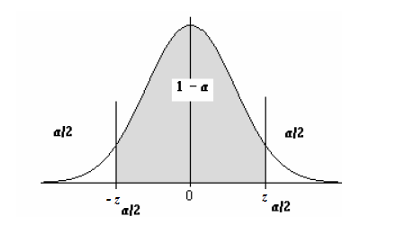
\includegraphics[scale=0.5]{Screenshot.png}
\end{center}

Per calcular el valor crític tenim en compte que si 
$$P\left(-z_{\alpha / 2} \leq Z \leq z_{\alpha / 2}\right)=1-\alpha$$llavors 
$$P\left(Z \geq z_{\alpha / 2}\right)=\frac{\alpha}{2}$$ (veure dibuix) i per tant 
$$P\left(Z \leq z_{\alpha / 2}\right)=1-\frac{\alpha}{2}$$ i això ho podem buscar a la taula de la $\mathrm{N}(0,1)$.\\
\end{concept}

\begin{exemple} \noindent
\textbf{Exemple}: Calcular el valor crític corresponent a un nivell de confiança del 99\%.

Com que 
$$1-\alpha=0,99 \Rightarrow \alpha=0,01 \Rightarrow \frac{\alpha}{2}=0,005 \Rightarrow 1-\frac{\alpha}{2}=0,995$$ 
I busquem ara a la taula el valor de $z$ que deixa a l'esquerra una probabilitat de 0,995, obtenint:

$$
z_{\alpha / 2}=2,575
$$
    
\end{exemple}

\begin{exercici} \noindent

\textbf{Exercici}: Calcula els valors crítics pel 90\%, 92\%, 95\%, 98\%, 99,5\%\\

Solucions: 

\begin{itemize}
    \item Nivell de confiança del 90\%:   $z_{\alpha / 2} = 1,645$
    \item Nivell de confiança del 92\%: $z_{\alpha / 2} = 1,751$
    \item Nivell de confiança del 95\%: $z_{\alpha / 2} = 1,960$
    \item Nivell de confiança del 98\%: $z_{\alpha / 2} = 2,326$
    \item Nivell de confiança del 99,5\%: $z_{\alpha / 2} = 2,807$
\end{itemize}
    
\end{exercici}



\subsection{Interval de confiança per la mitjana poblacional}

\begin{concept} [title=Concepte] \noindent
   
Suposem que la població de partida és $N(\mu, \sigma)$, i volem estimar mitjançant un interval la mitjana de la població, $\mu$, que és desconeguda. Per a això escollim una mostra aleatòria de mida $n$ i calculem la mitjana mostral, $\bar{X}$.

Com vam veure en el tema anterior, la mitjana mostral té una distribució coneguda:

$$
\bar{X} \rightarrow N\left(\mu, \frac{\sigma}{\sqrt{n}}\right)
$$

I per tant, tipificant: $\quad Z=\dfrac{\bar{X}-\mu}{\sigma / \sqrt{n}} \rightarrow N(0,1)$
Fixat un nivell de confiança, $1-\alpha$, volem dos valors tals que la probabilitat que la mitjana de la població, $\mu$, es trobi entre ells sigui precisament $1-\alpha$.

Si ens fixem en la definició de valor crític:

$$
P\left(-z_{\alpha / 2} \leq Z \leq z_{\alpha / 2}\right)=1-\alpha
$$

D'on

$$
P\left(-z_{\alpha / 2} \leq \frac{\bar{X}-\mu}{\sigma / \sqrt{n}} \leq z_{\alpha / 2}\right)=1-\alpha
$$

Despejant:

$$
P\left(-z_{\alpha / 2} \cdot \sigma / \sqrt{n} \leq \bar{X}-\mu \leq z_{\alpha / 2} \cdot \sigma / \sqrt{n}\right)=1-\alpha
$$

I per tant:

$$
P\left(\bar{X}-z_{\alpha / 2} \cdot \sigma / \sqrt{n} \leq \mu \leq \bar{X}+z_{\alpha / 2} \cdot \sigma / \sqrt{n}\right)=1-\alpha
$$

És a dir:
L'interval de confiança per al paràmetre $\mu$ d'una població $N(\mu, \sigma)$ al nivell de confiança $1-\alpha$ ve donat per:


\begin{center}
\doublebox{
\(
\left(\bar{X}-z_{\alpha / 2} \cdot \sigma / \sqrt{n}, \bar{X}+z_{\alpha / 2} \cdot \sigma / \sqrt{n}\right)
\)
}
\end{center}


Nota: Si $\sigma$ es desconeguda, es substitueix per la desviació típica de la mostra, \textit{S}.\\

Definirem \textbf{error màxim admisible} com:

\begin{center}
\doublebox{\(E = z_{\alpha / 2} \cdot \dfrac{\sigma}{\sqrt{n}}
\)}
\end{center}
\end{concept}

\begin{exemple} [title=Exemple 1:] \noindent
Se sap que la desviació típica de les talles dels alumnes d'una universitat és de 5 cm. Es desitja estimar la talla mitjana d'aquests alumnes, per la qual cosa es tria una mostra de 100 estudiants i s'obté que la mitjana mostral és de 172 cm. \\

Trobar l'interval de confiança per a la talla mitjana de la universitat per als nivells de confiança del 90 i del $95 \%$.\\

\textbf{Solució}:
Tenim $\sigma=5, \mathrm{n}=100$ i $\bar{x}=172$

\begin{itemize}
    \item Calculem el valor crític per al nivell de confiança del 90\%:


$$
1-\alpha=0,90 \Rightarrow \alpha=0,1 \Rightarrow \frac{\alpha}{2}=0,05 \Rightarrow 1-\frac{\alpha}{2}=0,95
$$

I busquem ara a la taula el valor de z que deixa a l'esquerra una probabilitat de 0,95, obtenint (aprox.):  $z_{\alpha / 2}=1,64$


Substituint en la fórmula de l'interval de confiança:

$$
\begin{aligned}
& \left(\bar{X}-z_{\alpha / 2} \cdot \sigma / \sqrt{n}, \bar{X}+z_{\alpha / 2} \cdot \sigma / \sqrt{n}\right) \\
& 172-1,64 \cdot \frac{5}{\sqrt{100}}=172-0,82=171,18 \\
& 172+1,64 \cdot \frac{5}{\sqrt{100}}=172+0,82=172,82
\end{aligned}
$$

Llavors l'interval de confiança per al $90 \%$ serà: \doublebox{$IC_{90}=\left(171,18, 172,82\right)$}\\

\item Fem el mateix per al nivell de confiança del 95\%:

$$
1-\alpha=0,99 \Rightarrow \alpha=0,01 \Rightarrow \frac{\alpha}{2}=0,005 \Rightarrow 1-\frac{\alpha}{2}=0,995
$$

I busquem ara a la taula el valor de z que deixa a l'esquerra una probabilitat de 0,995, obtenint (aprox.):$z_{\alpha / 2}=2,58$


Substituint en la fórmula de l'interval de confiança:

$$
\begin{aligned}
& \left(\bar{X}-z_{\alpha / 2} \cdot \sigma / \sqrt{n}, \bar{X}+z_{\alpha / 2} \cdot \sigma / \sqrt{n}\right) \\
& 172-2,58 \cdot \frac{5}{\sqrt{100}}=172-1,29=170,71 \\
& 172+2,58 \cdot \frac{5}{\sqrt{100}}=172+1,29=173,29
\end{aligned}
$$


Llavors l'interval de confiança per al $99 \%$ serà: \doublebox{$IC_{99}=\left(170,71,173,29\right)$}
\end{itemize}

\end{exemple}

\begin{exemple} [title=Exemple 2:] \noindent

Un psicòleg escolar vol estimar la mitjana de temps de reacció a un determinat estímul dels alumnes de $1^{\circ}$ de Primària. Per a això ha triat una mostra de 35 nens obtenint un temps mitjà de 1,12 minuts i una desviació típica de $0,21$ minuts.\\ 

Trobar l'interval de confiança per al temps mitjà de reacció amb un nivell de significació del 8\%.\\

\textbf{Solució:}
Com que $n$ és gran, podem usar la fórmula de l'interval de confiança usant la desviació típica mostral ja que desconeixem la de la població:

$$
\left(\bar{X}-z_{\alpha / 2} \cdot s / \sqrt{n}, \bar{X}+z_{\alpha / 2} \cdot s / \sqrt{n}\right)
$$

Tenim $s=0,21, \mathrm{n}=35$ i $\bar{x}=1,12$\\

Calculem el valor crític per al nivell de confiança del $92 \%$ (ja que $\alpha=0,08$):

$$
1-\alpha=0,92 \Rightarrow \alpha=0,08 \Rightarrow \frac{\alpha}{2}=0,04 \Rightarrow 1-\frac{\alpha}{2}=0,96
$$

I busquem ara a la taula el valor de $z$ que deixa a l'esquerra una probabilitat de 0,96, obtenint (aprox.): $z_{\alpha / 2}=1,75$\\

Llavors:

$$
\begin{aligned}
& 1,12-1,75 \cdot \frac{0,21}{\sqrt{35}}=1,12-0,06=1,06 \\
& 1,12+1,75 \cdot \frac{0,21}{\sqrt{35}}=1,12+0,06=1,18
\end{aligned}
$$

I per tant l'interval de confiança serà: \doublebox{$\quad IC_{92}=\left(1,06,1,18\right)$}
\end{exemple}

\subsection{Interval de confiança per la proporció}

\begin{concept} [title= Concepte] \noindent
Ara desitgem estimar la proporció $p$ amb la qual una determinada característica es dóna en una població. Per a això extraiem una mostra de mida $n$ i obtenim la proporció mostral, és a dir,

$$
\hat{p}=\frac{\text{número d'individus que compleixen la característica}}{\text{mida de la mostra}}
$$\\

Com vam veure en el tema anterior, la distribució de les proporcions mostrals és:

$$
\hat{P} \rightarrow N\left(p, \sqrt{\frac{p q}{n}}\right)
$$

on $q=1-p$\\

Donat un nivell de confiança, $1-\alpha$, i fent el mateix que en el cas de la mitjana, s'obté el següent interval de confiança per a la proporció de la població:

\begin{center}
\doublebox{
\(
\left(\hat{p}-z_{\alpha / 2} \cdot \sqrt{\dfrac{\hat{p} \hat{q}}{n}}, \; \;\hat{p}+z_{\alpha / 2} \cdot \sqrt{\dfrac{\hat{p} \hat{q}}{n}}\right)\)}
\end{center}

Pel que fa al erro màxim admisible:

\begin{center}
\doublebox{
\(
E =\left (z_{\alpha / 2} \cdot \sqrt{\dfrac{\hat{p} \hat{q}}{n}}\right)
\)}
\end{center}
\end{concept}

\begin{exemple} [title=Exemple 1] \noindent
Prenent a l'atzar una mostra de 300 persones majors de 15 anys en una gran ciutat, es troba que 104 d'elles llegien el diari habitualment. \\

Trobar, amb un nivell de confiança del $90 \%$, un interval per estimar la proporció de lectors de diari entre els habitants d'aquesta ciutat majors de 15 anys.\\
    
\end{exemple}

\begin{exemple} [title=] \noindent

\textbf{Solució:}

La proporció mostral és: $\hat{p}=\dfrac{104}{300}=0,347$
El valor crític per a un nivell de confiança del $90 \%$:

$$
1-\alpha=0,90 \Rightarrow \alpha=0,1 \Rightarrow \frac{\alpha}{2}=0,05 \Rightarrow 1-\frac{\alpha}{2}=0,95
$$

Llavors $z_{\alpha / 2}=1,64$
Llavors substituint en la fórmula: $\left(\hat{p}-z_{\alpha / 2} \cdot \sqrt{\dfrac{\hat{p} \hat{q}}{n}}, \hat{p}+z_{\alpha / 2} \cdot \sqrt{\dfrac{\hat{p} \hat{q}}{n}}\right)$

$$
\begin{aligned}
& 0,347-1,64 \cdot \sqrt{\frac{0,347 \cdot 0,653}{300}}=0,347-0,045=0,302 \\
& 0,347+1,64 \cdot \sqrt{\frac{0,347 \cdot 0,653}{300}}=0,347+0,045=0,392
\end{aligned}
$$

Llavors l'interval demanat és \doublebox{$IC_{90}=\left(0,302,0,392\right)$}
\end{exemple}

\begin{exemple} [title=Exemple 2] \noindent
    \textbf{Exemple 2:}

De què mida hauríem de triar una mostra per estimar la proporció d'alumnes de l'institut que els agrada el futbol amb un nivell de confiança del 95\% i un error inferior a 0,05, si en una mostra de 10 alumnes, 6 d'ells van respondre que els agradava el futbol?\\


\textbf{Solució:}

Tenim:
\begin{itemize}
    \item Mida de la mostra inicial: $n = 10$
    \item Proporció mostral: $\hat{p} = \dfrac{6}{10} = 0,6$
    \item Nivell de confiança: $95\%$
    \item Error màxim: $0,05$
\end{itemize}

El valor crític per a un nivell de confiança del 95\% és $z_{\alpha / 2} = 1,96$.\\

El càlcul de la mida de la mostra necessària és:
$$
n = \left(\dfrac{z_{\alpha / 2}^2 \cdot \hat{p} \cdot (1 - \hat{p})}{\text{error màxim}^2}\right)
$$

Substituint els valors:
$$
n = \left(\dfrac{1,96^2 \cdot 0,6 \cdot (1 - 0,6)}{0,05^2}\right) = 368,79
$$

Per tant, la mida de la mostra necessària és:
$$
n = 369
$$
\end{exemple}

\begin{exercici} [title= Llistat d'exercicis] \noindent
  \begin{enumerate}
      \item \href{https://drive.google.com/file/d/1EWxzhZPnZKRB6bLXsgMgLqGI-WuRvcpV/view?usp=drive_link}{\textbf{Enunciats}} 
      \item \href{https://drive.google.com/file/d/1CcdnZ5pccXwBpPzfIMhqTmCC_bdsnXOO/view?usp=drive_link}{\textbf{Solucions}}
  \end{enumerate}  
\end{exercici}

\end{document}
